\documentclass[12pt]{report}
\usepackage[a4paper,
    left=0.7in,
    right=0.7in,
    top=1.5in,
    bottom=1in,
    headheight=15pt,
    headsep=0.5in,
    footskip=0.5in
]{geometry}
\usepackage{fancyhdr}
\usepackage{tabularx}
\usepackage{longtable}
\usepackage{enumitem}
\usepackage{tocloft}
\usepackage{booktabs}
\usepackage{ragged2e}
\usepackage{hyperref}
\usepackage{tikz}
\usepackage{dashrule}
\usepackage{xcolor}
\usepackage{graphicx}
\usepackage{pmboxdraw}
\usepackage{float}
\usepackage{rotating}
\usepackage{placeins}
\usepackage{setspace}
\usepackage{titling}
\usepackage{titlesec}
\usepackage{algorithm}
\usepackage{algpseudocode}
\usepackage{amsmath}
\usepackage{listings}

% Listings configuration for Python code
\lstset{
  language=Python,
  basicstyle=\ttfamily\footnotesize,
  keywordstyle=\color{blue}\bfseries,
  commentstyle=\color{gray}\itshape,
  stringstyle=\color{red},
  numbers=left,
  numberstyle=\tiny\color{gray},
  stepnumber=1,
  numbersep=8pt,
  backgroundcolor=\color{white},
  showspaces=false,
  showstringspaces=false,
  showtabs=false,
  frame=single,
  tabsize=4,
  captionpos=b,
  breaklines=true,
  breakatwhitespace=false,
  escapeinside={(*@}{@*)},
  xleftmargin=2em,
  framexleftmargin=1.5em
}

% Chapter Formatting
\titleformat{\chapter}[display]
  {\centering\bfseries\fontsize{18}{20}\selectfont}
  {Chapter \thechapter}
  {0pt}
  {}

\titlespacing*{\chapter}
  {0pt}
  {0pt}
  {12pt}

% Enable deep numbering
\setcounter{secnumdepth}{3}
\setcounter{tocdepth}{3}

% Header & Footer Setup
\pagestyle{fancy}
\fancyhf{}
\fancyhead[L]{\small COMSATS University Islamabad}
\fancyhead[R]{\small Software Requirements Specification}
\fancyfoot[C]{\thepage}
\renewcommand{\headrulewidth}{0.4pt}
\renewcommand{\footrulewidth}{0pt}

\begin{document}

% ---- Title Page ----
\begin{titlepage}
\centering
\vspace*{2cm}
{\Large\bfseries COMSATS University Islamabad\par}
\vspace{0.5cm}
{\large Department of Computer Science\par}
\vspace{2cm}
{\Huge\bfseries Software Requirements Specification\par}
\vspace{0.5cm}
{\LARGE Quantum Virtual Machine (QVM)\par}
\vspace{1cm}
{\large A Hardware-Agnostic Quantum Circuit Execution Platform\par}
\vspace{2cm}
{\large Final Year Project\par}
\vspace{3cm}
{\large\today\par}
\end{titlepage}

% ---- Table of Contents ----
\pagenumbering{roman}
\tableofcontents
\newpage
\listoffigures
\newpage
\listoftables

% ---- Main Content ----
\clearpage
\pagenumbering{arabic}

% Chapter 1: Introduction (provides context for the SRS)
% ==============================
% Chapter 1 – Introduction
% ==============================

\chapter{Introduction}

% --------------------------------
% 1.1 Introduction
% --------------------------------

\section{Introduction}

Quantum computing represents a paradigm shift in computational capability, promising exponential speedups for specific classes of problems including cryptography, optimization, and molecular simulation. Unlike classical computers that process information using binary bits, quantum computers leverage quantum mechanical phenomena such as superposition and entanglement to perform computations on quantum bits (qubits). This fundamental difference enables quantum algorithms to solve certain problems that are intractable for classical computers, positioning quantum computing as a transformative technology for the 21st century.

However, the quantum computing ecosystem currently faces a critical challenge: hardware fragmentation. Major quantum hardware vendors including IBM, Google, Rigetti, and IonQ employ fundamentally different physical implementations—superconducting qubits, trapped ions, photonic systems, and neutral atoms—each with unique native gate sets, qubit connectivity topologies, and error characteristics. This diversity, while beneficial for exploring different technological approaches, creates significant barriers for software developers. A quantum algorithm optimized for IBM's heavy-hex topology cannot execute efficiently on Google's Sycamore architecture without substantial manual refactoring. This vendor lock-in problem mirrors the early days of classical computing before standardized instruction sets and operating systems emerged.

Current industry practice requires quantum developers to write hardware-specific code, manually decompose gates into target-specific primitives, and explicitly manage qubit routing to satisfy connectivity constraints. This low-level programming model significantly increases development complexity and reduces code portability. Existing quantum software development kits (SDKs) such as Qiskit, Cirq, and PyQuil are tightly coupled to their respective hardware platforms, offering limited abstraction and requiring developers to understand intricate hardware details. While these frameworks provide powerful capabilities, they lack a unified middleware layer that enables true "Write Once, Run Anywhere" (WORA) functionality.

The absence of hardware abstraction creates several critical inefficiencies. First, algorithm developers must maintain multiple implementations of the same quantum circuit for different hardware platforms, increasing maintenance burden and introducing potential inconsistencies. Second, researchers cannot easily compare algorithm performance across different quantum architectures, hindering objective evaluation of hardware capabilities. Third, educational institutions face challenges teaching quantum programming when students must learn platform-specific details rather than focusing on algorithmic concepts. Fourth, the quantum software ecosystem remains fragmented, with limited code reuse and collaboration across different hardware communities.

These challenges motivated the development of the Quantum Virtual Machine (QVM), a hardware-agnostic quantum execution runtime that implements the WORA philosophy for quantum computing. The QVM serves as an abstraction layer between high-level quantum algorithms and diverse hardware backends, automatically handling the complex tasks of gate decomposition, qubit mapping, and circuit optimization. By accepting quantum programs in standardized formats (OpenQASM 2.0, OpenQASM 3.0, JSON) and transpiling them for arbitrary hardware topologies, the QVM enables developers to write quantum algorithms once and execute them on any supported backend without modification.

The proposed system addresses hardware fragmentation through a comprehensive compilation pipeline encompassing parsing, intermediate representation, decomposition, topology-aware transpilation, and high-fidelity simulation. The QVM provides both exact statevector simulation for small-scale circuits and efficient Matrix Product State (MPS) simulation for larger low-entanglement systems, enabling algorithm validation before deployment to real quantum hardware. This approach not only solves the immediate portability problem but also establishes a foundation for future quantum software development practices, analogous to how Java Virtual Machine (JVM) and LLVM transformed classical software development by providing hardware abstraction and code portability.



% --------------------------------
% 1.2 Vision Statement
% --------------------------------

\section{Vision Statement}

The Quantum Virtual Machine envisions a future where quantum algorithm developers, researchers, and educators can focus on algorithmic innovation rather than hardware-specific implementation details. Our target stakeholders include quantum software developers seeking code portability across diverse quantum platforms, academic institutions requiring accessible quantum computing education tools, and research organizations conducting comparative studies of quantum algorithms across different hardware architectures.

The core problem we address is the fundamental lack of hardware abstraction in the quantum computing ecosystem, which forces developers to maintain multiple platform-specific implementations of the same algorithm, creates vendor lock-in, and impedes the growth of a unified quantum software community. This fragmentation mirrors the early days of classical computing before standardized instruction sets and virtual machines emerged to enable true code portability.

Our long-term vision is to establish the QVM as a foundational middleware layer for quantum computing, analogous to how the Java Virtual Machine (JVM) transformed classical software development by decoupling application logic from underlying hardware. We envision a quantum software ecosystem where algorithms are written once in standardized formats and automatically optimized for any quantum hardware backend, enabling seamless migration between platforms as technology evolves.

The innovation of this system lies in its comprehensive approach to hardware abstraction, combining advanced transpilation algorithms with dual simulation engines to provide both exact verification and scalable approximate simulation. By automating gate decomposition, topology-aware qubit routing, and circuit optimization, the QVM reduces the barrier to entry for quantum programming while enabling experienced developers to leverage sophisticated compilation techniques without manual intervention.

The strategic impact extends beyond immediate code portability: by establishing patterns for hardware-agnostic quantum software development, the QVM contributes to the maturation of quantum computing as a field, accelerating the transition from hardware-centric to software-centric quantum algorithm development and fostering a collaborative ecosystem where quantum software can be shared, reused, and improved across the entire quantum computing community.



% --------------------------------
% 1.3 Related System Analysis
% --------------------------------

\section{Related System Analysis}

The quantum software development landscape is dominated by several major frameworks, each with distinct strengths and limitations. Understanding these existing systems is crucial for positioning the QVM's contributions and identifying areas for improvement.

\textbf{Qiskit (IBM Quantum)} represents the industry standard for quantum programming, offering the most comprehensive suite of tools for quantum algorithm development. Qiskit provides extensive libraries for quantum chemistry, optimization, machine learning, and finance applications. Its transpiler supports sophisticated optimization passes including gate cancellation, commutation analysis, and layout optimization. The framework integrates seamlessly with IBM's cloud-based quantum processors and provides pulse-level control for fine-grained hardware manipulation. However, Qiskit's comprehensiveness comes at a cost: the installation footprint exceeds 500MB with numerous dependencies, creating a steep learning curve for beginners. The framework is tightly coupled with IBM's ecosystem, and while it theoretically supports other backends through plugins, the primary focus remains IBM hardware. The extensive abstraction layers, while powerful, can obscure the underlying quantum operations, making it challenging for educational purposes where transparency is essential.

\textbf{Cirq (Google Quantum AI)} focuses on near-term quantum algorithms and circuit optimization for Google's quantum processors. Cirq emphasizes explicit circuit construction with fine-grained control over gate placement and timing. The framework provides excellent support for variational quantum algorithms and includes built-in noise modeling capabilities. Cirq's design philosophy prioritizes transparency and control, making it popular among researchers who need precise circuit specification. However, this low-level approach requires developers to manually handle many details that other frameworks automate. The framework lacks the extensive algorithm libraries found in Qiskit, and its primary optimization target is Google's Sycamore architecture. While Cirq can export to OpenQASM for cross-platform compatibility, the conversion process may not preserve all circuit optimizations, and the framework provides limited support for hardware topologies significantly different from Google's grid-based architecture.

\textbf{ProjectQ (ETH Zurich)} pioneered many concepts in quantum compilation and emulation, featuring a sophisticated compiler engine with automatic gate decomposition and circuit optimization. ProjectQ's architecture separates the high-level quantum programming interface from backend-specific compilation, demonstrating early recognition of the hardware abstraction problem. The framework supports multiple backends including simulators and real hardware through a plugin system. However, ProjectQ's development has slowed in recent years, with the last major release predating many recent advances in quantum compilation. The framework's architecture, while innovative for its time, lacks support for modern features such as OpenQASM 3.0, advanced control flow, and hybrid classical-quantum computation. The documentation and community support have diminished compared to more actively maintained frameworks, making it less suitable for new projects despite its technical merits.

\textbf{PyQuil (Rigetti Computing)} implements the Quil instruction set and emphasizes hybrid quantum-classical algorithms through its Quantum Abstract Machine (QAM) model. PyQuil provides excellent support for parametric compilation and real-time classical control, making it well-suited for variational algorithms and quantum-classical feedback loops. The framework's integration with Rigetti's quantum cloud services enables seamless execution on real hardware. However, PyQuil is primarily designed for Rigetti's specific chip architectures, and while it supports other backends through adapters, the framework's design assumptions reflect Rigetti's hardware characteristics. The Quil instruction set, while powerful, represents yet another platform-specific language that developers must learn, contributing to ecosystem fragmentation rather than solving it.

The proposed QVM addresses limitations across these existing systems by providing a lightweight, educational-focused implementation that prioritizes transparency, hardware agnosticism, and ease of use. Unlike Qiskit's heavy installation footprint, the QVM maintains minimal dependencies (NumPy, Lark, FastAPI) totaling under 50MB. Unlike Cirq's low-level approach, the QVM automates complex transpilation tasks while remaining transparent about the transformations applied. Unlike ProjectQ's aging architecture, the QVM supports modern standards including OpenQASM 3.0 with full control flow. Unlike PyQuil's platform-specific focus, the QVM treats all hardware topologies equally, with no preferential optimization for any particular vendor. The QVM's dual simulation architecture (statevector and MPS) provides both exact verification and scalable approximate simulation, a combination not found in any single existing framework.

\vspace{0.5cm}

\begin{table}[h!]
\centering
\caption{Comparative Analysis of Existing Systems}
\renewcommand{\arraystretch}{1.3}

\begin{tabularx}{\textwidth}{|p{3cm}|X|X|}
\hline
\textbf{Application Name} & \textbf{Identified Weaknesses} & \textbf{Proposed Improvements} \\
\hline
Qiskit (IBM) &
\begin{itemize}[leftmargin=*, noitemsep, topsep=0pt]
    \item Heavy installation (500+ MB)
    \item Steep learning curve
    \item IBM ecosystem coupling
    \item Complex abstraction layers
\end{itemize}
&
\begin{itemize}[leftmargin=*, noitemsep, topsep=0pt]
    \item Lightweight (<50 MB)
    \item Educational focus
    \item True hardware agnosticism
    \item Transparent pipeline
\end{itemize}
\\
\hline
Cirq (Google) &
\begin{itemize}[leftmargin=*, noitemsep, topsep=0pt]
    \item Manual low-level control required
    \item Limited algorithm libraries
    \item Google architecture focus
    \item Verbose circuit construction
\end{itemize}
&
\begin{itemize}[leftmargin=*, noitemsep, topsep=0pt]
    \item Automated transpilation
    \item Built-in algorithms
    \item Topology-agnostic design
    \item Concise circuit specification
\end{itemize}
\\
\hline
ProjectQ (ETH) &
\begin{itemize}[leftmargin=*, noitemsep, topsep=0pt]
    \item Development stagnation
    \item No OpenQASM 3.0 support
    \item Limited control flow
    \item Aging architecture
\end{itemize}
&
\begin{itemize}[leftmargin=*, noitemsep, topsep=0pt]
    \item Active development
    \item Full OpenQASM 3.0 support
    \item Advanced control flow
    \item Modern architecture
\end{itemize}
\\
\hline
PyQuil (Rigetti) &
\begin{itemize}[leftmargin=*, noitemsep, topsep=0pt]
    \item Rigetti-specific design
    \item Quil language lock-in
    \item Limited cross-platform support
    \item Vendor coupling
\end{itemize}
&
\begin{itemize}[leftmargin=*, noitemsep, topsep=0pt]
    \item Hardware-agnostic design
    \item Standard formats (OpenQASM)
    \item Universal backend support
    \item Vendor independence
\end{itemize}
\\
\hline

\end{tabularx}
\end{table}



% --------------------------------
% 1.4 Project Deliverables
% --------------------------------

\section{Project Deliverables}

The Quantum Virtual Machine project delivers a comprehensive suite of software components, documentation artifacts, and validation materials that collectively demonstrate a complete quantum compilation and simulation system. Each deliverable serves a specific purpose in achieving the project's objectives of hardware abstraction and code portability.

\textbf{List of Deliverables:}

\begin{enumerate}
    \item \textbf{Core QVM Engine} – The central compilation and simulation system comprising six integrated modules: Parser, Intermediate Representation (IR), Decomposer, Transpiler, Simulator, and Visualizer. The engine accepts quantum circuits in multiple formats (OpenQASM 2.0, OpenQASM 3.0, JSON), performs hardware-agnostic compilation, and executes circuits using either exact statevector or approximate MPS simulation. This deliverable includes full support for classical memory integration, conditional operations, and advanced control flow (loops, jumps, labels), enabling hybrid quantum-classical algorithm execution.

    \item \textbf{Parser Module} – A robust parsing system built on the Lark parsing toolkit, providing AST-based parsing for OpenQASM 2.0 and 3.0 with comprehensive grammar coverage. The parser handles quantum gate declarations, qubit and classical bit registers, measurement operations, conditional statements, for/while loops, and timing directives. The module validates circuit syntax, performs semantic analysis, and generates the internal IR representation. A JSON parser provides backward compatibility with simple gate list formats.

    \item \textbf{Transpilation System} – An advanced compilation module implementing both greedy BFS routing and SABRE-inspired lookahead heuristics for topology-aware qubit mapping. The transpiler automatically inserts SWAP gates to satisfy hardware connectivity constraints, supports configurable routing strategies, and provides optional mapping restoration to preserve logical-physical qubit correspondence. The system includes architecture definitions for linear and grid topologies with extensibility for custom hardware configurations.

    \item \textbf{Dual Simulation Engine} – Two complementary simulation backends: (1) Statevector Simulator providing exact quantum state evolution for circuits up to 12 qubits using NumPy vectorization and permutation-based gate application, supporting all standard gates plus Toffoli, and (2) MPS Simulator implementing tensor network simulation with SVD-based compression for low-entanglement circuits scaling to 20+ qubits. Both simulators support mid-circuit measurements with state collapse, classical memory operations, and conditional gate execution.

    \item \textbf{Command-Line Interface (CLI)} – A comprehensive command-line tool providing access to all QVM functionality through an intuitive interface. The CLI supports circuit loading from files, configurable transpilation with routing strategy selection, simulation parameter tuning (seed, max operations), visualization options, and detailed output formatting. The interface includes extensive help documentation and error reporting to guide users through quantum program execution.

    \item \textbf{Web API and Dashboard} – A FastAPI-based RESTful web service enabling remote circuit submission and execution, with JSON request/response formatting for easy integration with external applications. The accompanying web dashboard provides an interactive interface for circuit composition, parameter configuration, execution monitoring, and result visualization. The web interface demonstrates the QVM's capability as a backend service for quantum computing applications.

    \item \textbf{Visualization Module} – A Matplotlib-based visualization system generating publication-quality circuit diagrams with proper gate symbols, qubit lines, and measurement indicators. The module produces probability histograms for measurement outcomes, supports customizable styling, and enables export to various image formats. Visualization aids in algorithm debugging, educational demonstrations, and result presentation.

    \item \textbf{Comprehensive Documentation} – Extensive technical documentation including system architecture descriptions, module API references, algorithm explanations (Bernstein-Vazirani, Grover's search), usage guides for CLI and web interfaces, and example quantum programs. Documentation artifacts include this Software Requirements Specification (SRS), Software Design Document (SDD), test reports, and user manuals ensuring system maintainability and accessibility.

    \item \textbf{Automated Test Suite} – A comprehensive pytest-based testing framework with 36 automated tests covering unit testing (individual module validation), integration testing (inter-module communication), and system testing (end-to-end algorithm execution). The test suite validates simulator correctness through quantum algorithm verification, transpiler functionality through connectivity constraint checking, and parser robustness through malformed input handling.

    \item \textbf{Example Quantum Algorithms} – Implemented and verified quantum algorithms demonstrating QVM capabilities: Bell state preparation, GHZ state generation, Bernstein-Vazirani hidden string finding, and Grover's search algorithm. Each example includes circuit generators, expected output verification, and performance benchmarks, serving as both validation tests and educational resources.

    \item \textbf{Deployment Package} – A complete installation package with dependency specifications (requirements.txt), setup instructions, configuration files, and deployment scripts for local and server environments. The package includes all source code, tests, documentation, and examples necessary for independent QVM deployment and operation.
\end{enumerate}

These deliverables collectively provide a production-ready quantum virtual machine suitable for educational use, algorithm research, and quantum software development, fulfilling all project objectives outlined in the scope document.



% --------------------------------
% 1.5 System Limitations / Constraints
% --------------------------------

\section{System Limitations / Constraints}

The Quantum Virtual Machine, while providing comprehensive quantum compilation and simulation capabilities, operates within several technical and practical constraints that define its operational boundaries and use cases.

\textbf{Qubit Scalability Constraints:} The statevector simulator faces fundamental exponential memory limitations, requiring $2^n$ complex numbers (16 bytes each) to represent an $n$-qubit quantum state. This restricts practical simulation to approximately 12 qubits on standard hardware with 16GB RAM, as a 13-qubit state requires 128KB and a 20-qubit state would require 16MB of memory just for the state vector. While the MPS simulator extends this range to 20+ qubits for low-entanglement circuits, highly entangled quantum states cause exponential bond dimension growth, negating the compression benefits and reverting to exponential resource requirements.

\textbf{Ideal Simulation Model:} The current implementation assumes perfect, noiseless quantum operations without modeling realistic hardware imperfections. Real quantum devices suffer from decoherence (T1 relaxation), dephasing (T2 relaxation), gate errors (typically 0.1-1\% for single-qubit gates, 1-5\% for two-qubit gates), and measurement errors (1-5\%). The absence of noise modeling means simulation results represent idealized behavior that may significantly differ from actual hardware execution, particularly for deep circuits where errors accumulate. This limitation restricts the system's utility for predicting real-world quantum algorithm performance on NISQ devices.

\textbf{Transpiler Optimality:} The qubit routing problem is NP-hard, and the implemented heuristic algorithms (greedy BFS and SABRE) do not guarantee optimal SWAP insertion or minimal circuit depth. While SABRE typically achieves 30-40\% depth reduction compared to greedy routing, both approaches may produce circuits with more SWAP gates than theoretically necessary. This suboptimality increases circuit execution time and, on real hardware, amplifies error accumulation due to additional gate operations.

\textbf{Hardware Topology Support:} The current architecture definitions primarily support regular topologies (linear chains, 2D grids). More complex real-world topologies such as IBM's heavy-hex lattice, Google's Sycamore grid with specific connectivity patterns, or Rigetti's Aspen architecture require additional configuration. The routing algorithms assume bidirectional connectivity and may require modification for hardware with directional coupling or asymmetric gate fidelities.

\textbf{Classical Computation Overhead:} Transpilation and simulation introduce significant classical computational overhead. SABRE routing complexity scales as $O(G \cdot E \cdot L)$ where $G$ is the number of gates, $E$ is the number of edges in the connectivity graph, and $L$ is the lookahead depth. Statevector simulation requires $O(2^n)$ operations per gate. For small problem instances, this classical overhead may exceed any theoretical quantum speedup, making the system primarily suitable for algorithm development and validation rather than production quantum computation.

\textbf{Software and Hardware Dependencies:} The system requires Python 3.10+ and depends on NumPy for numerical computation, Lark for parsing, and FastAPI for web services. These dependencies, while minimal compared to frameworks like Qiskit, still impose version compatibility requirements. The system is designed for x86-64 architecture and has not been optimized for ARM processors or specialized hardware accelerators (GPUs, TPUs).

\textbf{Deployment and Integration Constraints:} The QVM currently operates as a standalone application without native cloud deployment, job queuing, or multi-user support. Integration with real quantum hardware requires manual circuit export to OpenQASM and external submission to vendor-specific platforms. The system does not include authentication, authorization, or resource management features necessary for production multi-tenant environments.

Despite these limitations, the QVM successfully demonstrates hardware-agnostic quantum computing principles and provides a valuable tool for quantum algorithm education, development, and validation within its operational constraints.



% --------------------------------
% 1.6 Tools and Technologies
% --------------------------------

\section{Tools and Technologies}

The Quantum Virtual Machine leverages a carefully selected technology stack that balances functionality, performance, and maintainability while minimizing dependencies and installation complexity. Each technology choice reflects specific technical requirements and design principles.

\textbf{Python 3.10+} serves as the core programming language, selected for its extensive scientific computing ecosystem, readable syntax suitable for educational purposes, and widespread adoption in the quantum computing community. Python's dynamic typing and high-level abstractions enable rapid development while maintaining code clarity. The 3.10+ requirement ensures access to modern language features including structural pattern matching and improved type hints.

\textbf{NumPy} provides the foundation for all numerical computation, offering highly optimized linear algebra operations through BLAS/LAPACK backends. NumPy's vectorized operations enable efficient statevector manipulation, with gate application achieving near-C performance through compiled routines. The library's array broadcasting and advanced indexing capabilities are essential for implementing permutation-based gate operations in the simulator.

\textbf{Lark} implements the parsing infrastructure, providing a pure-Python parsing toolkit with LALR(1) parser generation from EBNF grammars. Lark's choice over alternatives like PLY or ANTLR reflects its lightweight footprint, excellent error reporting, and native Python integration. The toolkit enables full OpenQASM 3.0 support through a formal grammar specification, ensuring robust parsing with clear error messages.

\textbf{FastAPI} powers the web service layer, offering modern asynchronous request handling with automatic OpenAPI documentation generation. FastAPI's Pydantic integration provides automatic request validation and serialization, while its ASGI foundation enables high-performance concurrent request processing. The framework's minimal boilerplate and intuitive routing make it ideal for exposing QVM functionality as a RESTful API.

\textbf{Matplotlib} handles all visualization requirements, generating publication-quality circuit diagrams and probability histograms. Matplotlib's extensive customization options and multiple backend support (interactive, file export) make it suitable for both educational demonstrations and research presentations.

\textbf{pytest} provides the testing framework, offering powerful fixture management, parametrized testing, and comprehensive assertion introspection. The framework's plugin ecosystem and clear test organization support the 36-test suite covering unit, integration, and system-level validation.

\textbf{Git and GitHub} manage version control and collaboration, with Git providing distributed version control and GitHub offering issue tracking, pull request workflows, and continuous integration hooks. The repository structure follows Python best practices with clear module organization and comprehensive documentation.

\textbf{VS Code} serves as the primary development environment, selected for its excellent Python support through extensions, integrated debugging, Git integration, and terminal access. The editor's lightweight nature and cross-platform compatibility make it accessible to all developers.

The technology stack intentionally avoids heavy dependencies like TensorFlow or PyTorch, keeping the total installation footprint under 50MB compared to 500+ MB for frameworks like Qiskit. This minimalist approach aligns with the project's educational focus and ensures rapid deployment on resource-constrained systems.

\begin{table}[h!]
\centering
\caption{Tools and Technologies Used in the Project}
\renewcommand{\arraystretch}{1.3}
\begin{tabularx}{\textwidth}{|p{4cm}|p{3cm}|X|}
\hline
\textbf{Tool / Technology} & \textbf{Version} & \textbf{Purpose} \\
\hline
Python & 3.10+ & Core programming language for all system components \\
\hline
NumPy & 1.24+ & Linear algebra operations, statevector manipulation, gate application \\
\hline
Lark & 1.1+ & OpenQASM parsing, AST generation, grammar-based validation \\
\hline
FastAPI & 0.100+ & RESTful web service, asynchronous request handling, API documentation \\
\hline
Matplotlib & 3.7+ & Circuit visualization, probability histograms, result plotting \\
\hline
pytest & 7.4+ & Automated testing framework, unit/integration test execution \\
\hline
Git & 2.40+ & Version control, code history, branch management \\
\hline
GitHub & N/A & Repository hosting, issue tracking, collaboration platform \\
\hline
VS Code & 1.80+ & Integrated development environment, debugging, code editing \\
\hline
NetworkX & 3.1+ & Graph algorithms for topology analysis and routing \\
\hline
\end{tabularx}
\end{table}




% --------------------------------
% 1.7 Relevance to Course Modules
% --------------------------------

\section{Relevance to Course Modules}

\textbf{Writing Guidelines (400–600 words total)}

\begin{itemize}
    \item Demonstrate integration of academic knowledge into practical implementation.
    \item Reflect on how theoretical concepts were applied.
    \item Connect specific course modules to project components.
    \item Highlight achievement of learning outcomes.
\end{itemize}

\vspace{0.5cm}

\subsection{Programming Fundamentals}

The QVM implementation extensively applies object-oriented programming principles learned in Programming Fundamentals courses. The system architecture employs class-based design with clear encapsulation: the \texttt{QuantumCircuit} class encapsulates circuit state and operations, the \texttt{Simulator} class manages quantum state evolution, and the \texttt{Transpiler} class handles qubit routing logic. Inheritance is demonstrated through the dual simulator architecture, where both \texttt{Simulator} and \texttt{MPSSimulator} implement a common interface for circuit execution. Modular design principles guide the six-module pipeline architecture (Parser, IR, Decomposer, Transpiler, Simulator, Visualizer), with each module maintaining single responsibility and loose coupling through well-defined interfaces. Control flow concepts including loops, conditionals, and exception handling are applied throughout, particularly in the parser's AST traversal and the transpiler's iterative SWAP insertion algorithm. The project demonstrates practical application of algorithmic thinking, data structure selection, and code organization principles essential to software development.


\subsection{Data Structures and Algorithms}

The QVM leverages advanced data structures and algorithms studied in DSA courses. Graph algorithms form the foundation of the transpiler: the hardware topology is represented as an undirected graph using adjacency lists, and Breadth-First Search (BFS) computes shortest paths between qubits for SWAP insertion. The SABRE routing algorithm implements a sophisticated heuristic optimization technique with lookahead evaluation and decay mechanisms to minimize circuit depth. Hash tables (Python dictionaries) provide O(1) lookup for gate definitions, qubit mappings, and classical memory registers. The MPS simulator employs tensor data structures with dynamic array resizing and Singular Value Decomposition (SVD) for state compression. Priority queues guide the transpiler's gate selection during routing. The parser constructs Abstract Syntax Trees (ASTs) using recursive descent, demonstrating tree traversal algorithms. These implementations showcase practical application of algorithmic complexity analysis, optimization techniques, and appropriate data structure selection for performance-critical quantum computing operations.


\subsection{Database Management Systems}

The Quantum Virtual Machine does not employ traditional relational database systems, as the application operates as a stateless computational engine processing quantum circuits without persistent data storage requirements. The system's architecture focuses on in-memory computation rather than data persistence: quantum states are represented as NumPy arrays in RAM, circuit definitions are parsed from files on-demand, and simulation results are returned directly to users without database storage. Classical memory within quantum circuits (classical bits and registers) is managed through in-memory hash tables rather than database tables. While database concepts such as data normalization and relationship modeling informed the design of the Intermediate Representation (IR) schema, the project's computational nature and educational focus prioritized algorithmic efficiency over data persistence. Future extensions could incorporate databases for job queuing, user management, or result archiving in multi-user deployment scenarios.


\subsection{Software Engineering}

Software Engineering principles permeate the entire QVM development lifecycle. The project follows an iterative development model with incremental feature delivery across three major phases: Phase 1 (core simulation), Phase 2 (transpilation and OpenQASM 3.0), and Phase 3 (web interface and optimization). Comprehensive UML diagrams document system design: Use Case diagrams identify stakeholders and interactions, Class diagrams specify object relationships, Sequence diagrams illustrate execution flows, Activity diagrams model algorithmic processes, and State diagrams capture circuit lifecycle transitions. The requirements engineering process produced 48 functional requirements and 24 non-functional requirements with full traceability to business objectives. The testing strategy implements a three-tier approach: 36 unit tests validate individual modules, integration tests verify inter-module communication, and system tests confirm end-to-end algorithm execution. Version control through Git enables collaborative development and change tracking. This systematic application of SDLC methodologies, documentation standards, and quality assurance practices demonstrates professional software engineering competency.


\subsection{Other Relevant Courses}

The QVM integrates knowledge from multiple specialized courses beyond core computer science curriculum. \textbf{Linear Algebra} forms the mathematical foundation: quantum states are represented as complex vectors in Hilbert space, gate operations are unitary matrices, and the simulator performs matrix-vector multiplication for state evolution. Concepts of eigenvalues, tensor products, and basis transformations are essential to quantum computation. \textbf{Quantum Computing} courses provided the theoretical framework for qubit superposition, entanglement, measurement collapse, and quantum algorithms (Grover's search, Bernstein-Vazirani). \textbf{Compiler Design} principles inform the transpilation pipeline: lexical analysis (tokenization), syntax analysis (parsing), semantic analysis (type checking), and code optimization (SWAP minimization) mirror classical compiler stages. \textbf{Web Development} knowledge enabled the FastAPI-based RESTful service and interactive dashboard. \textbf{Numerical Methods} guided the implementation of SVD-based tensor compression in the MPS simulator. This interdisciplinary integration demonstrates the synthesis of mathematical, physical, and computational concepts in quantum software engineering.

%%%%%%%%%%%%%%%%%%%%%%%%%%%%%%%%%%%%%%%%%%%%%%%%%%%%%%
\section{Chapter Summary}
%%%%%%%%%%%%%%%%%%%%%%%%%%%%%%%%%%%%%%%%%%%%%%%%%%%%%%

This chapter introduced the background and context of the proposed system, 
highlighting existing challenges and the need for improvement within the 
selected problem domain. The vision and strategic objectives of the system 
were outlined to establish its intended impact and innovation. A comparative 
analysis of related systems identified key limitations in current solutions. 
Project deliverables, system constraints, selected technologies, and academic 
relevance were also discussed. 

This chapter establishes the foundation for the detailed problem definition 
presented in the next chapter.


% Chapter 2: Problem Definition / Feasibility Study
% ==============================
% Chapter 2 – Problem Definition
% ==============================

\chapter{Problem Definition}
% --------------------------------
% 2.1 Problem Statement
% --------------------------------

\section{Problem Statement}

The primary problem this project addresses is \textbf{hardware fragmentation} and \textbf{vendor lock-in} in the quantum computing domain. Currently, quantum hardware providers use different underlying technologies (e.g., Superconducting Qubits vs. Trapped Ions), which result in incompatible instruction sets and connectivity graphs. A developer writing code for one platform often cannot run it on another without significant manual refactoring. Furthermore, optimizing a circuit for a specific device's topology is a complex, error-prone task that requires deep knowledge of the hardware. There is a lack of lightweight, educational, and open-source runtimes that demonstrate how to abstract these complexities effectively. This project aims to solve these interoperability challenges by automating the translation process, thereby reducing development time, eliminating vendor dependencies, and lowering the barrier to entry for quantum computing education and research.



% --------------------------------
% 2.2 Proposed Solution Overview
% --------------------------------

\section{Proposed Solution Overview}

The proposed system solves the hardware fragmentation problem by introducing a middleware layer—the Quantum Virtual Machine (QVM). Instead of targeting a specific device, developers write code for the QVM, which follows a three-stage pipeline: (1) \textbf{Ingestion:} The system accepts a high-level circuit (OpenQASM 3.0, 2.0, or JSON) and converts it into a standardized Intermediate Representation (IR). (2) \textbf{Transpilation:} The core engine analyzes the target backend's constraints (native gates and topology), inserts SWAP gates where necessary, and decomposes complex gates into the target's primitive basis gates. (3) \textbf{Execution:} The system either executes the circuit on its internal hybrid simulator (Statevector or MPS) for verification or outputs the compiled circuit for a specific hardware target. This approach ensures that the logic of the algorithm remains preserved while the implementation details are automatically handled by the software, achieving true "Write Once, Run Anywhere" (WORA) functionality.



% --------------------------------
% 2.3 Objectives of the Proposed System
% --------------------------------

\section{Objectives of the Proposed System}

The following business objectives guide the development and evaluation of the Quantum Virtual Machine:

\vspace{0.3cm}

\textbf{Business Objectives (BO):}

\begin{itemize}
    \item \textbf{BO-1:} Develop a hardware-agnostic quantum execution runtime that enables developers to write quantum algorithms once and transpile them for different qubit topologies (Linear, Grid) without rewriting code.
    
    \item \textbf{BO-2:} Provide educational transparency into the transpilation process, showing users how logical qubits are mapped to physical ones and where SWAP gates are inserted to respect hardware constraints.
    
    \item \textbf{BO-3:} Implement a lightweight, standalone runtime suitable for local testing of small-scale quantum algorithms (up to 10-20 qubits) without requiring paid cloud subscriptions or enterprise dependencies.
    
    \item \textbf{BO-4:} Ensure interoperability by supporting OpenQASM 2.0 and 3.0 standards, making compiled circuits compatible with IBM quantum processors and other QASM-compliant platforms.
    
    \item \textbf{BO-5:} Automate the complex tasks of gate decomposition, qubit mapping, and circuit optimization through a robust transpilation pipeline, reducing manual effort and eliminating the need for deep hardware-specific knowledge.
\end{itemize}



% --------------------------------
% 2.4 Scope of the System
% --------------------------------

\section{Scope of the System}

The scope of this project is to develop a desktop-based Quantum Virtual Machine (QVM) using Python. The system will support the creation, compilation, and simulation of quantum circuits with a maximum capacity of 10-20 qubits depending on the simulation backend. The core functionality centers on a "Transpiler Pipeline" that accepts a high-level circuit definition (OpenQASM 3.0, 2.0, or JSON) and adapts it to specific architectural constraints (e.g., restricted connectivity). The system will support both Statevector simulation (exact linear algebra for up to 12 qubits) and MPS (Matrix Product States) simulation for low-entanglement circuits scaling to 20+ qubits. The output will include the final state vector, measurement probabilities, classical memory states, and visualized circuit diagrams. The project will \textbf{not} include pulse-level control, quantum error correction (QEC), or direct integration with real hardware APIs beyond OpenQASM string generation. The target users are quantum computing students, researchers, and educators requiring a lightweight, transparent, and educational quantum runtime environment.



% --------------------------------
% 2.5 System Architecture and Modules
% --------------------------------

\section{System Architecture and Modules}

The QVM follows a strict \textbf{Pipeline Architecture} pattern, ensuring clear separation of concerns and modular extensibility. The system processes quantum programs through six sequential stages: (1) \textbf{Input Layer:} Accepts OpenQASM 3.0, 2.0, or JSON gate lists. (2) \textbf{Parser (Lark):} Generates an Abstract Syntax Tree (AST) and maps it to the internal \texttt{QuantumCircuit} Intermediate Representation (IR). (3) \textbf{Decomposer:} Normalizes high-level gates into a target-compatible native gate set. (4) \textbf{Transpiler:} Routes qubits according to the target hardware topology using Greedy or SABRE routing algorithms. (5) \textbf{Simulators:} Executes the transpiled circuit using either the \texttt{Simulator} (exact statevector evolution) or \texttt{MPSSimulator} (tensor network contraction with SVD-based truncation). (6) \textbf{Output Layer:} Returns measurement probabilities, classical memory states, and visual plots. This modular design allows independent development, testing, and optimization of each component while maintaining a clean data flow from high-level quantum code to executable results.



% --------------------------------
% 2.5.1 Module Descriptions
% --------------------------------

\subsection{Module 1: Parser Module}

\textbf{Description}

The Parser Module serves as the entry point for quantum circuit ingestion, accepting programs in OpenQASM 2.0, OpenQASM 3.0, and JSON formats. Built on the Lark parsing toolkit, the module performs lexical analysis to tokenize input strings, syntactic analysis to construct Abstract Syntax Trees (ASTs) following formal grammar specifications, and semantic validation to ensure circuit correctness (valid qubit indices, supported gate types, proper register declarations). The parser handles advanced OpenQASM 3.0 features including classical memory operations, conditional execution, for/while loops, and timing directives. Upon successful parsing, the module generates the internal Intermediate Representation (IR) as a \texttt{QuantumCircuit} object containing structured gate sequences, qubit/classical bit registers, and metadata. Error handling provides detailed diagnostic messages with line numbers and syntax suggestions to guide users in correcting malformed circuits.

\textbf{Functional Requirements:}

\begin{itemize}
    \item FR-1.1: The system shall parse OpenQASM 2.0 circuits with support for standard gates (H, X, Y, Z, CNOT, CZ, SWAP, Toffoli) and measurement operations.
    \item FR-1.2: The system shall parse OpenQASM 3.0 circuits including classical memory declarations, conditional statements, and loop constructs.
    \item FR-1.3: The system shall validate circuit syntax and report errors with line numbers and descriptive messages.
    \item FR-1.4: The system shall generate an Intermediate Representation (IR) containing all circuit information in a standardized format.
    \item FR-1.5: The system shall support JSON circuit format for backward compatibility with simple gate list representations.
\end{itemize}



\subsection{Module 2: Transpiler Module}

\textbf{Description}

The Transpiler Module performs hardware-aware circuit compilation, transforming logical quantum circuits into physically executable programs that respect target hardware constraints. The module accepts a hardware topology specification (linear chain, 2D grid, or custom connectivity graph) and implements sophisticated qubit routing algorithms to satisfy connectivity requirements. The core functionality includes initial qubit placement using heuristic strategies, dynamic SWAP gate insertion to enable non-adjacent qubit interactions, and optional mapping restoration to preserve logical-physical qubit correspondence. The module supports two routing strategies: Greedy BFS for fast compilation with moderate optimization, and SABRE-inspired lookahead heuristics for superior circuit depth reduction (typically 30-40\% improvement). The transpiler integrates with the Decomposer to ensure all gates are expressed in the target's native gate set before routing, producing fully executable circuits ready for simulation or hardware deployment.

\textbf{Functional Requirements:}

\begin{itemize}
    \item FR-2.1: The system shall accept hardware topology specifications defining qubit connectivity constraints.
    \item FR-2.2: The system shall implement qubit routing algorithms (Greedy BFS and SABRE) to insert SWAP gates satisfying connectivity requirements.
    \item FR-2.3: The system shall minimize circuit depth and SWAP gate count through lookahead heuristics and decay mechanisms.
    \item FR-2.4: The system shall support configurable routing strategies allowing users to select optimization priorities.
    \item FR-2.5: The system shall provide optional mapping restoration to maintain logical-physical qubit correspondence after transpilation.
\end{itemize}



\subsection{Module 3: Simulator Module}

\textbf{Description}

The Simulator Module provides dual quantum state evolution engines for circuit execution and validation. The Statevector Simulator implements exact quantum mechanics using full state vector representation, supporting circuits up to 12 qubits on standard hardware through NumPy-optimized linear algebra operations. Gate application employs permutation-based indexing for efficient unitary matrix multiplication, achieving near-C performance through vectorized computation. The MPS (Matrix Product State) Simulator extends scalability to 20+ qubits for low-entanglement circuits using tensor network decomposition with SVD-based compression and configurable bond dimension truncation. Both simulators support mid-circuit measurements with probabilistic state collapse, classical memory operations (bit assignment, register manipulation), and conditional gate execution based on classical bit values. The module handles measurement sampling with configurable shot counts, probability distribution computation, and state vector extraction for analysis, providing comprehensive quantum circuit execution capabilities for algorithm development and validation.

\textbf{Functional Requirements:}

\begin{itemize}
    \item FR-3.1: The system shall simulate quantum circuits using exact statevector evolution for up to 12 qubits.
    \item FR-3.2: The system shall implement MPS simulation with SVD-based compression for low-entanglement circuits scaling to 20+ qubits.
    \item FR-3.3: The system shall support mid-circuit measurements with probabilistic state collapse and classical memory updates.
    \item FR-3.4: The system shall execute conditional gates based on classical bit values enabling hybrid quantum-classical algorithms.
    \item FR-3.5: The system shall compute measurement probability distributions and support configurable shot-based sampling.
\end{itemize}



\subsection{Module 4: Visualization Module}

\textbf{Description}

The Visualization Module generates publication-quality graphical representations of quantum circuits and simulation results using Matplotlib. The circuit diagram renderer produces professional visualizations with proper quantum gate symbols (boxes for single-qubit gates, controlled-gate notation for multi-qubit operations), horizontal qubit lines with clear labeling, measurement indicators, and classical bit wires. The module supports customizable styling including figure dimensions, color schemes, font sizes, and export formats (PNG, PDF, SVG) for integration into presentations and publications. Measurement result visualization includes probability histogram generation with configurable bar colors, axis labels, and statistical annotations. The module handles complex circuits with multiple qubits, classical registers, and conditional operations, automatically adjusting layout for readability. Visualization aids in algorithm debugging by revealing circuit structure, supports educational demonstrations by clarifying quantum operations, and enables result presentation through clear probability distributions.

\textbf{Functional Requirements:}

\begin{itemize}
    \item FR-4.1: The system shall generate circuit diagrams with proper quantum gate symbols and qubit line representations.
    \item FR-4.2: The system shall produce probability histograms visualizing measurement outcome distributions.
    \item FR-4.3: The system shall support customizable styling including colors, fonts, and figure dimensions.
    \item FR-4.4: The system shall export visualizations to multiple formats (PNG, PDF, SVG) for publication and presentation.
\end{itemize}



\subsection{Module 5: CLI and Web API Module}

\textbf{Description}

The CLI and Web API Module provides dual user interfaces for QVM access: a command-line interface for local execution and a RESTful web service for remote access. The CLI implements a comprehensive command-line tool with argument parsing for circuit file loading, transpilation configuration (routing strategy selection, topology specification), simulation parameters (seed, shot count, max operations), and output formatting options. The interface includes extensive help documentation, error reporting with actionable suggestions, and progress indicators for long-running operations. The Web API, built on FastAPI, exposes QVM functionality through HTTP endpoints with JSON request/response formatting, automatic OpenAPI documentation generation, and asynchronous request handling for concurrent circuit execution. The accompanying web dashboard provides an interactive interface for circuit composition, parameter configuration, execution monitoring, and result visualization, demonstrating the QVM's capability as a backend service for quantum computing applications and educational platforms.

\textbf{Functional Requirements:}

\begin{itemize}
    \item FR-5.1: The system shall provide a command-line interface accepting circuit files and configuration parameters.
    \item FR-5.2: The system shall implement a RESTful web API with JSON request/response formatting for remote circuit execution.
    \item FR-5.3: The system shall generate automatic API documentation using OpenAPI specifications.
    \item FR-5.4: The system shall provide an interactive web dashboard for circuit composition and result visualization.
    \item FR-5.5: The system shall support asynchronous request handling enabling concurrent circuit execution.
\end{itemize}


% --------------------------------
% 2.7 Assumptions and Dependencies
% --------------------------------

\section{Assumptions and Dependencies}

The following assumptions and dependencies guide the system design and operational constraints:

\textbf{Assumptions:}
\begin{itemize}
    \item The system assumes users have basic knowledge of quantum computing concepts (qubits, gates, superposition) and familiarity with Python programming.
    \item The system assumes quantum circuits are mathematically valid (unitary operations, proper qubit indexing) and syntactically correct according to OpenQASM specifications.
    \item The system assumes users have access to standard desktop hardware with at least 8GB RAM for simulating circuits up to 12 qubits (Statevector) or 20+ qubits (MPS for low-entanglement cases).
\end{itemize}

\textbf{Dependencies:}
\begin{itemize}
    \item The system depends on Python 3.10+ and core scientific libraries (NumPy for linear algebra, NetworkX for graph-based topology mapping, Matplotlib for visualization).
    \item The system depends on the Lark parsing library for OpenQASM 3.0 AST generation and syntax validation.
    \item The system's interoperability depends on adherence to OpenQASM 2.0 and 3.0 standards for circuit export and compatibility with external quantum platforms (e.g., IBM Quantum).
\end{itemize}

%%%%%%%%%%%%%%%%%%%%%%%%%%%%%%%%%%%%%%%%%%%%%%%%%%%%%%
\section{Chapter Summary}
%%%%%%%%%%%%%%%%%%%%%%%%%%%%%%%%%%%%%%%%%%%%%%%%%%%%%%

This chapter defined the core problem of hardware fragmentation and vendor lock-in in quantum computing, which prevents code portability across different quantum platforms. The proposed Quantum Virtual Machine (QVM) solution was presented as a middleware layer implementing a three-stage pipeline (Ingestion, Transpilation, Execution) to achieve "Write Once, Run Anywhere" functionality. Five clear business objectives were established to guide system development, focusing on hardware agnosticism, educational transparency, lightweight operation, interoperability, and automation. The system scope was defined to cover desktop-based quantum circuit simulation (10-20 qubits) using Python, with explicit boundaries excluding pulse-level control and quantum error correction. The pipeline architecture was outlined, describing the six-stage modular design from input parsing through simulation to output generation. Finally, key assumptions regarding user knowledge and hardware requirements, along with dependencies on Python libraries and OpenQASM standards, were documented to clarify operational constraints. This chapter provides the problem foundation and conceptual solution framework that will guide the detailed software design presented in the next chapter.


% Chapter 3: Requirement Analysis (core SRS content)
\chapter{Requirement Analysis}

\section{Introduction}
This chapter presents a comprehensive analysis of the requirements for the Quantum Virtual Machine (QVM) system. The requirements were gathered through a combination of literature review, analysis of existing quantum computing frameworks, and iterative prototyping. The chapter defines the functional and non-functional requirements that guided the system's design and implementation, ensuring that the QVM achieves its goal of providing a hardware-agnostic quantum execution runtime.

\section{Requirement Elicitation Techniques}
The requirements for the QVM were elicited using multiple complementary techniques to ensure comprehensive coverage of system needs:

\textbf{Literature Review:} Extensive analysis of academic papers and technical documentation from major quantum computing frameworks (Qiskit, Cirq, ProjectQ) to identify industry standards and best practices for quantum compilation and simulation.

\textbf{Comparative Analysis:} Systematic comparison of existing quantum SDKs to identify gaps in portability, educational accessibility, and hardware abstraction that the QVM aims to address.

\textbf{Prototyping and Iteration:} Incremental development approach where initial prototypes revealed technical constraints and user needs, leading to refined requirements for classical memory integration, control flow support, and transpilation strategies.

\textbf{Domain Expert Consultation:} Regular discussions with the FYP supervisor and review of quantum computing research to validate technical requirements and ensure alignment with quantum computing principles.

\section{User Classes and Characteristics}

\begin{table}[H]
\centering
\caption{User Classes and Characteristics}
\begin{tabular}{|p{3cm}|p{5cm}|p{5cm}|}
\hline
\textbf{User Class} & \textbf{Description} & \textbf{Characteristics} \\
\hline
Quantum Algorithm Developers & Users who write and test quantum algorithms & Technical background in quantum computing; need hardware abstraction; require visualization and debugging tools \\
\hline
Students and Educators & Academic users learning quantum computing concepts & Beginner to intermediate technical skills; need clear documentation; require educational examples and visual feedback \\
\hline
Researchers & Users conducting quantum computing research & Advanced technical skills; need flexibility and extensibility; require accurate simulation and performance metrics \\
\hline
System Integrators & Users integrating QVM with other tools & Software engineering background; need API access; require export capabilities (OpenQASM) \\
\hline
\end{tabular}
\end{table}

\section{System Overview}
The Quantum Virtual Machine is a comprehensive quantum circuit execution platform that implements a complete compilation and simulation pipeline. The system accepts quantum programs in multiple formats (OpenQASM 2.0, OpenQASM 3.0, JSON), transforms them through a hardware-agnostic intermediate representation, applies topology-aware transpilation, and executes them using either exact statevector simulation or efficient tensor network methods. The system provides three user interfaces (CLI, Web API, Web GUI) to accommodate different usage scenarios, from automated scripting to interactive exploration. The architecture emphasizes modularity, allowing each component (parser, transpiler, simulator) to be independently tested and upgraded.

\section{Use Case Model}
This section defines the primary interactions between the actors and the Quantum Virtual Machine system, capturing the functional requirements from a user-centric perspective.

\subsection{Combined Use Case Diagram}
The use case diagram in Figure \ref{fig:use_case_diagram} provides a high-level visual overview of the system's functionality and all actors involved.

\begin{figure}[H]
\centering
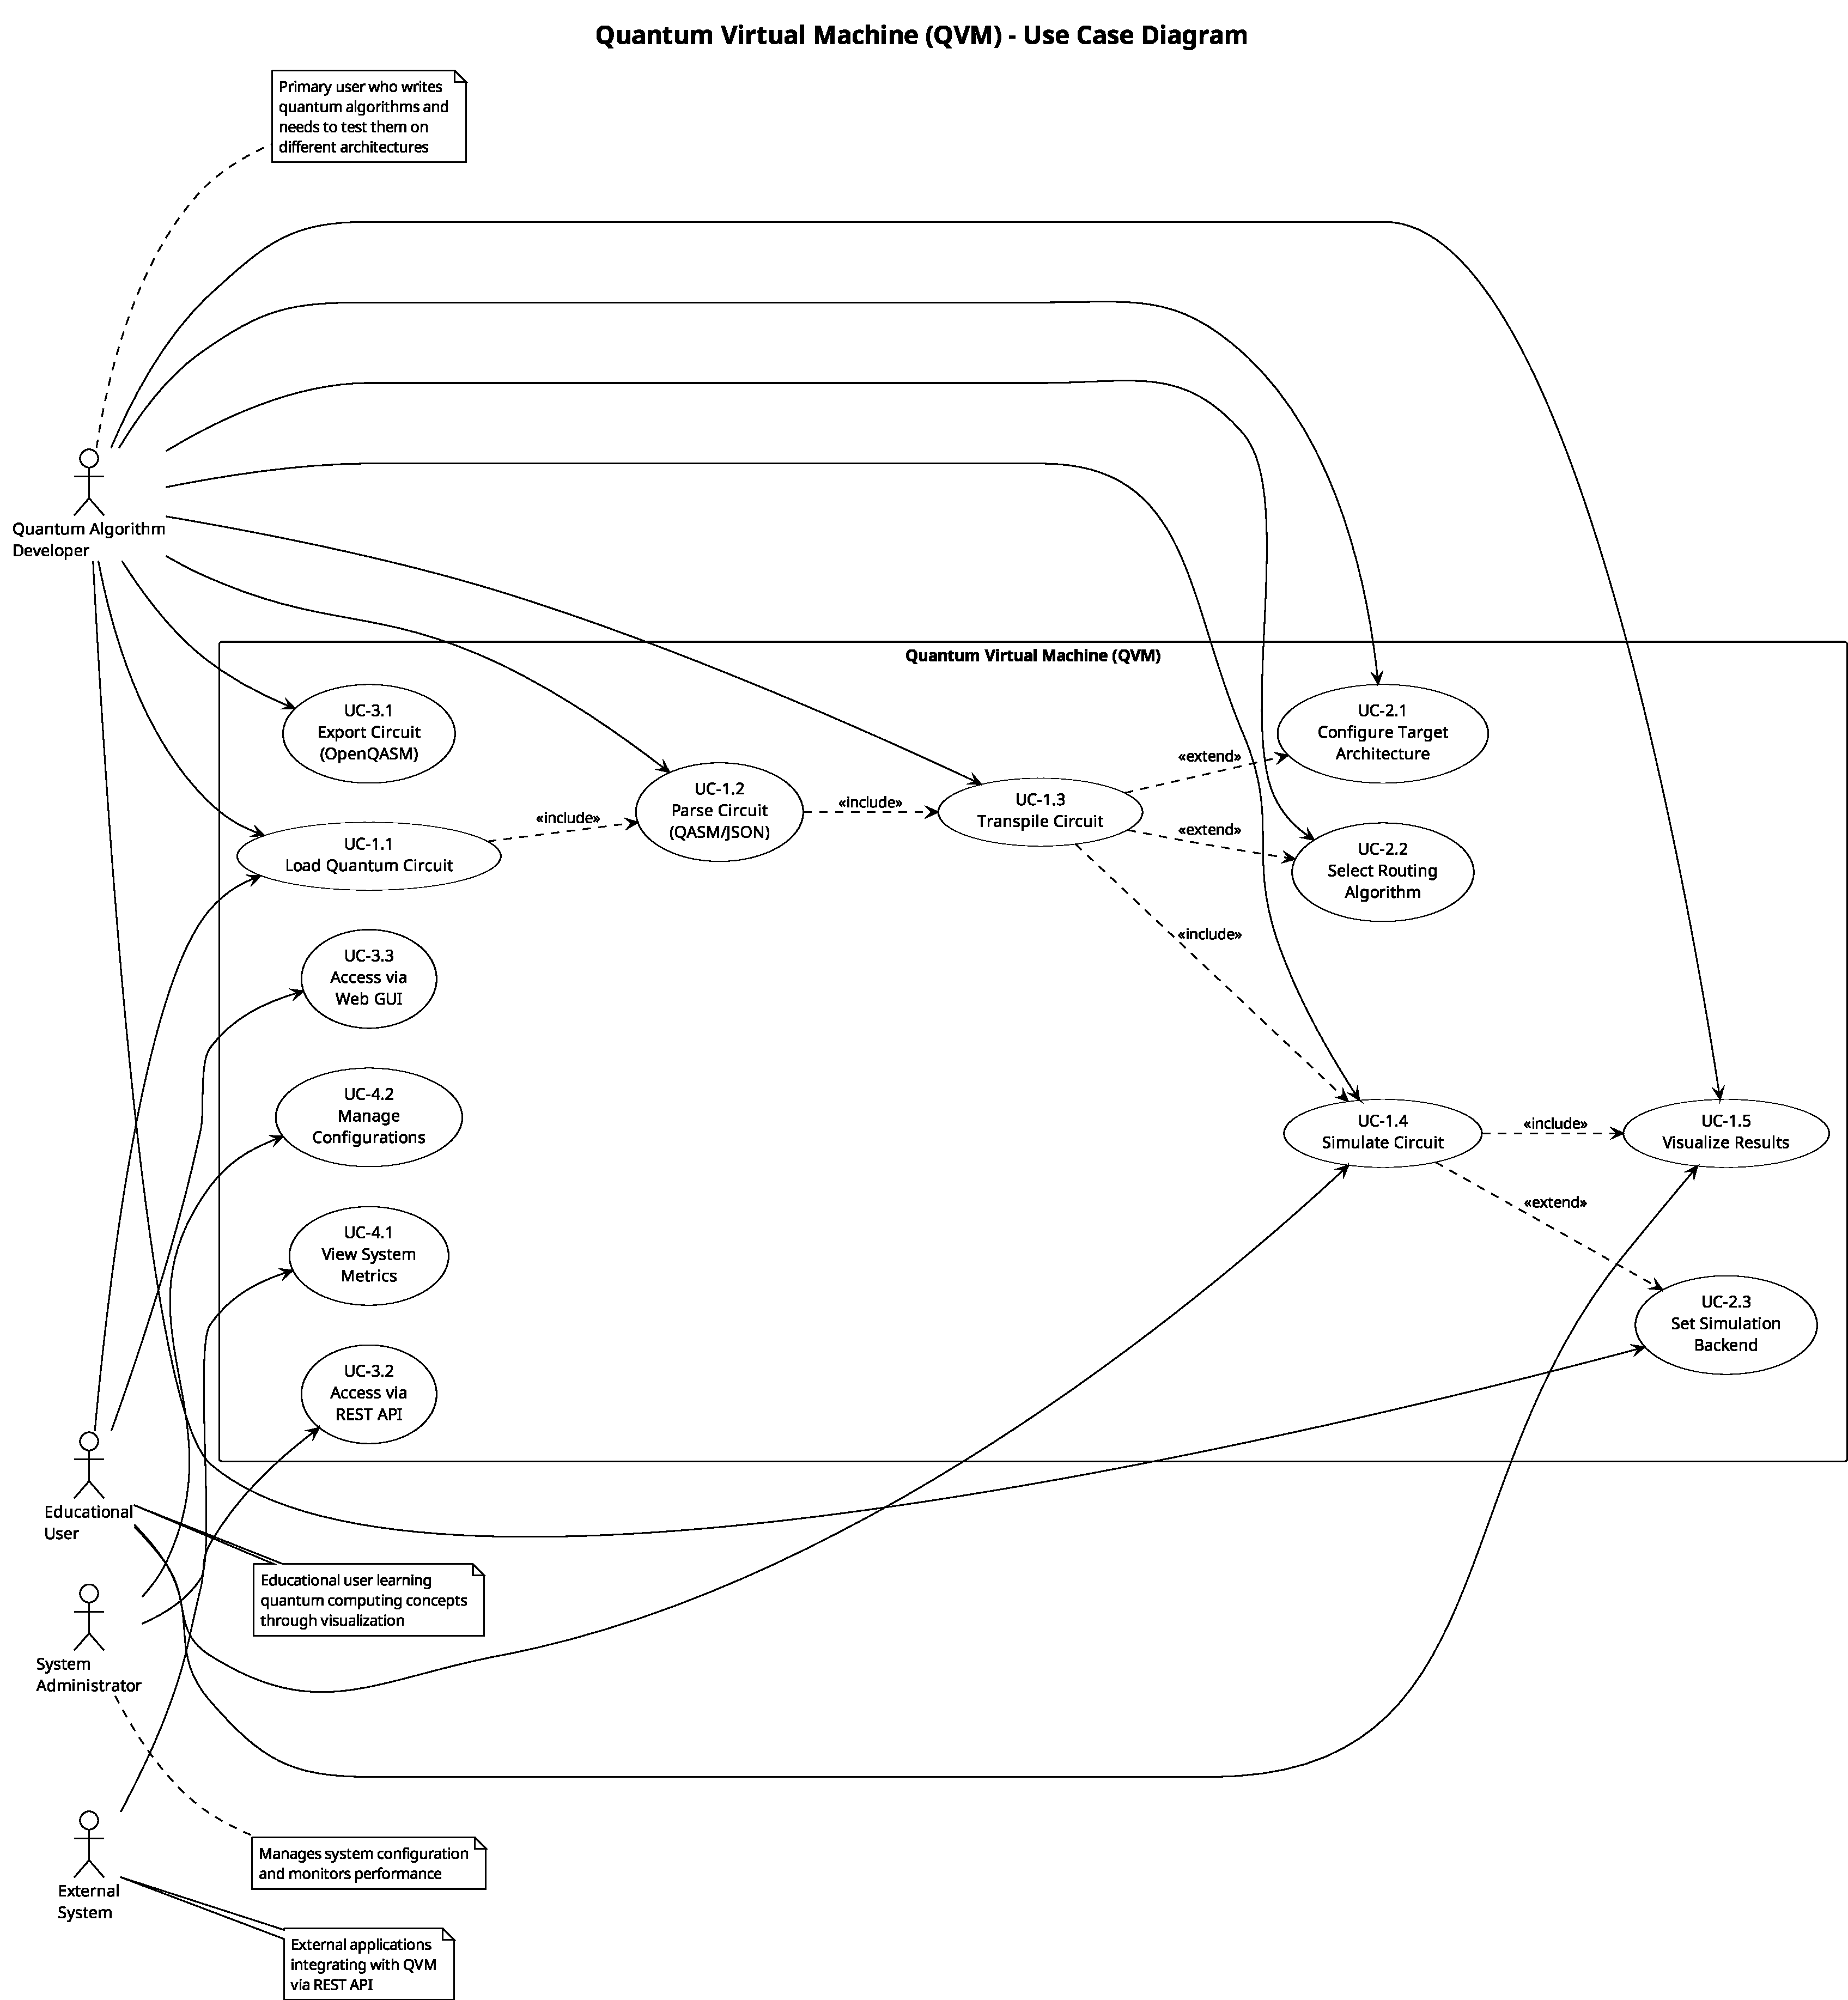
\includegraphics[width=0.9\textwidth,height=0.8\textheight,keepaspectratio]{../uml/QVM_Use_Case_Diagram.pdf}
\caption{Combined Use Case Diagram for Quantum Virtual Machine}
\label{fig:use_case_diagram}
\end{figure}

\subsection{Actor-Specific Use Case Diagrams}
The following diagrams present individual use case views for each distinct user class, showing the specific interactions and system capabilities relevant to each actor.

\subsubsection{Quantum Algorithm Developer}
Figure \ref{fig:uc_developer} illustrates the use cases available to the Quantum Algorithm Developer. This actor is the primary user of the system, interacting with the QVM to parse, transpile, simulate, and visualize quantum circuits via the command-line interface.

\begin{figure}[H]
\centering
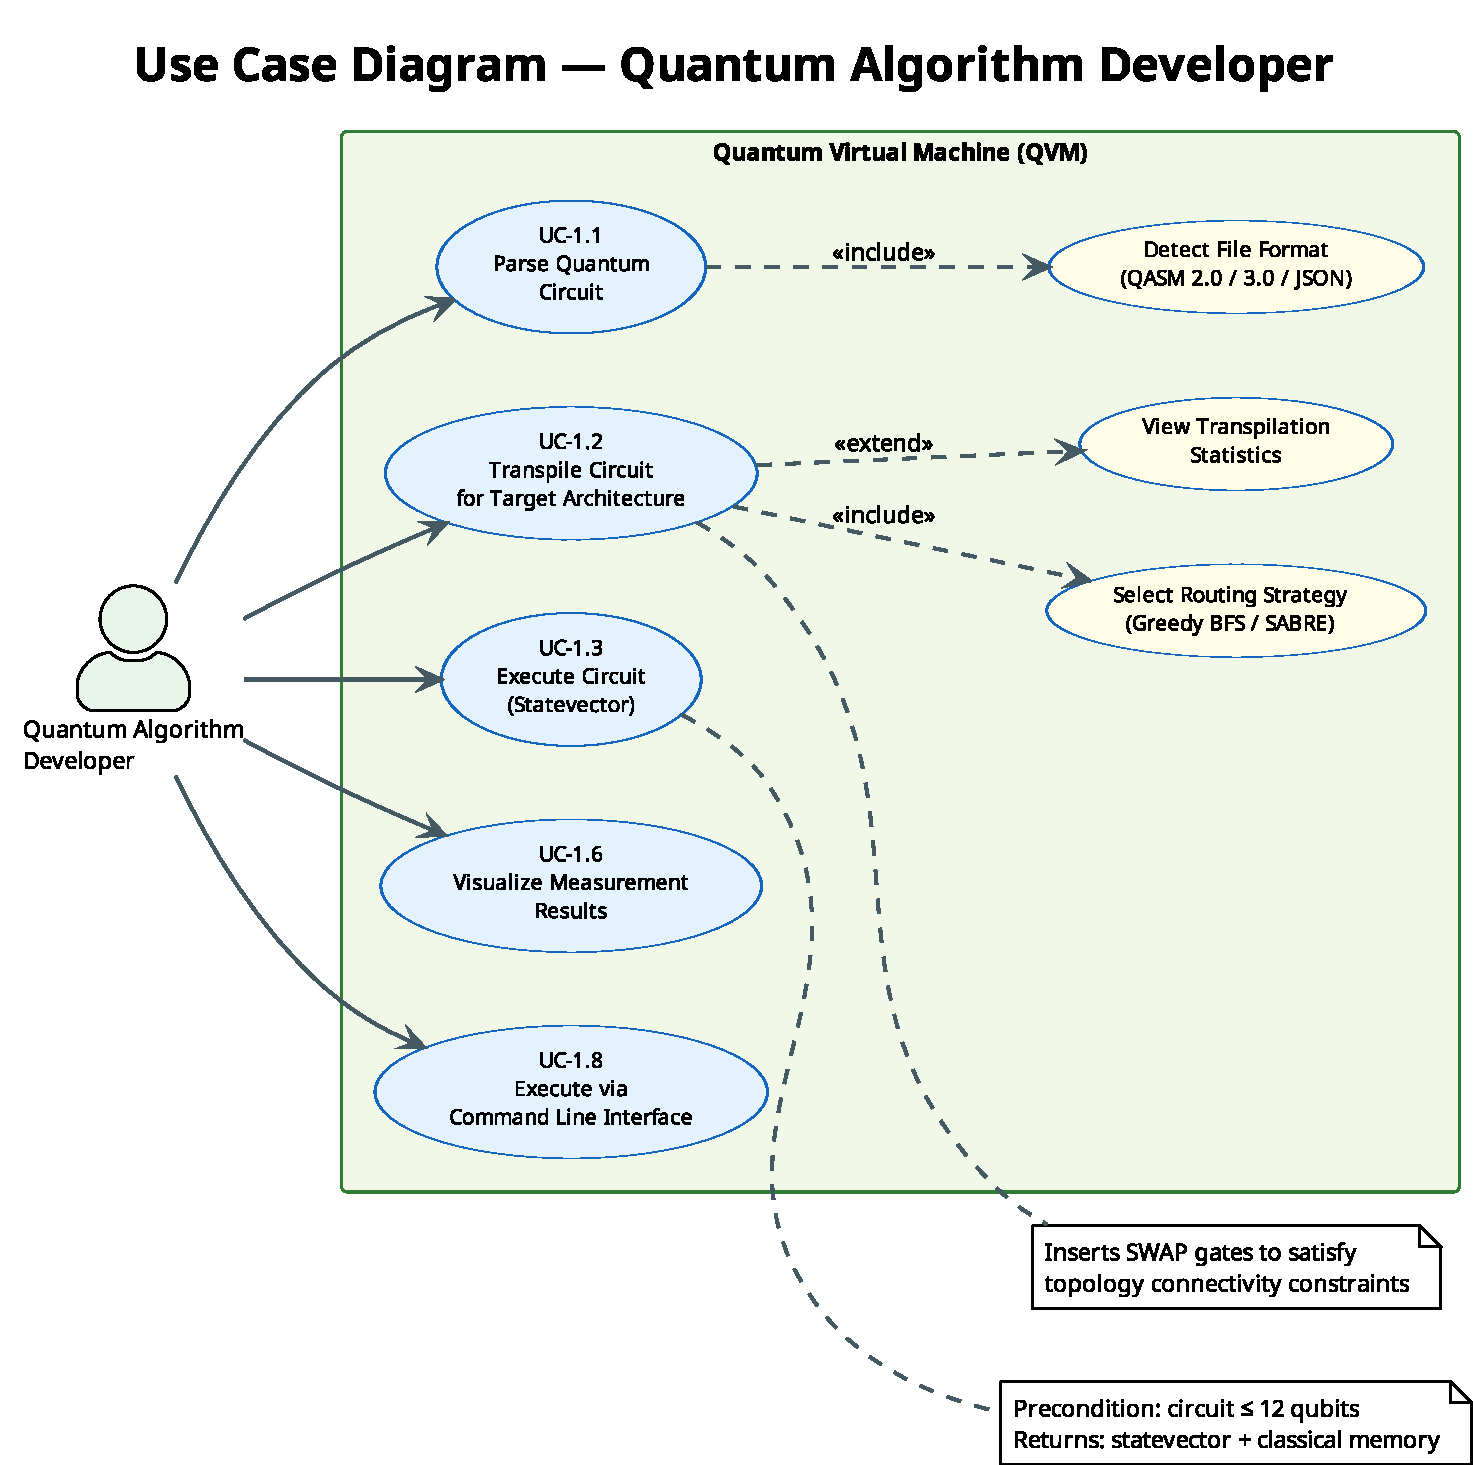
\includegraphics[width=0.9\textwidth,height=0.75\textheight,keepaspectratio]{../standalone_docs/figures/UC_Developer.pdf}
\caption{Use Case Diagram --- Quantum Algorithm Developer}
\label{fig:uc_developer}
\end{figure}

\subsubsection{Student / Educator}
Figure \ref{fig:uc_student} shows the use cases for the Student / Educator actor. This user class interacts primarily with the web-based GUI and visualization features to learn quantum computing concepts through experimentation.

\begin{figure}[H]
\centering
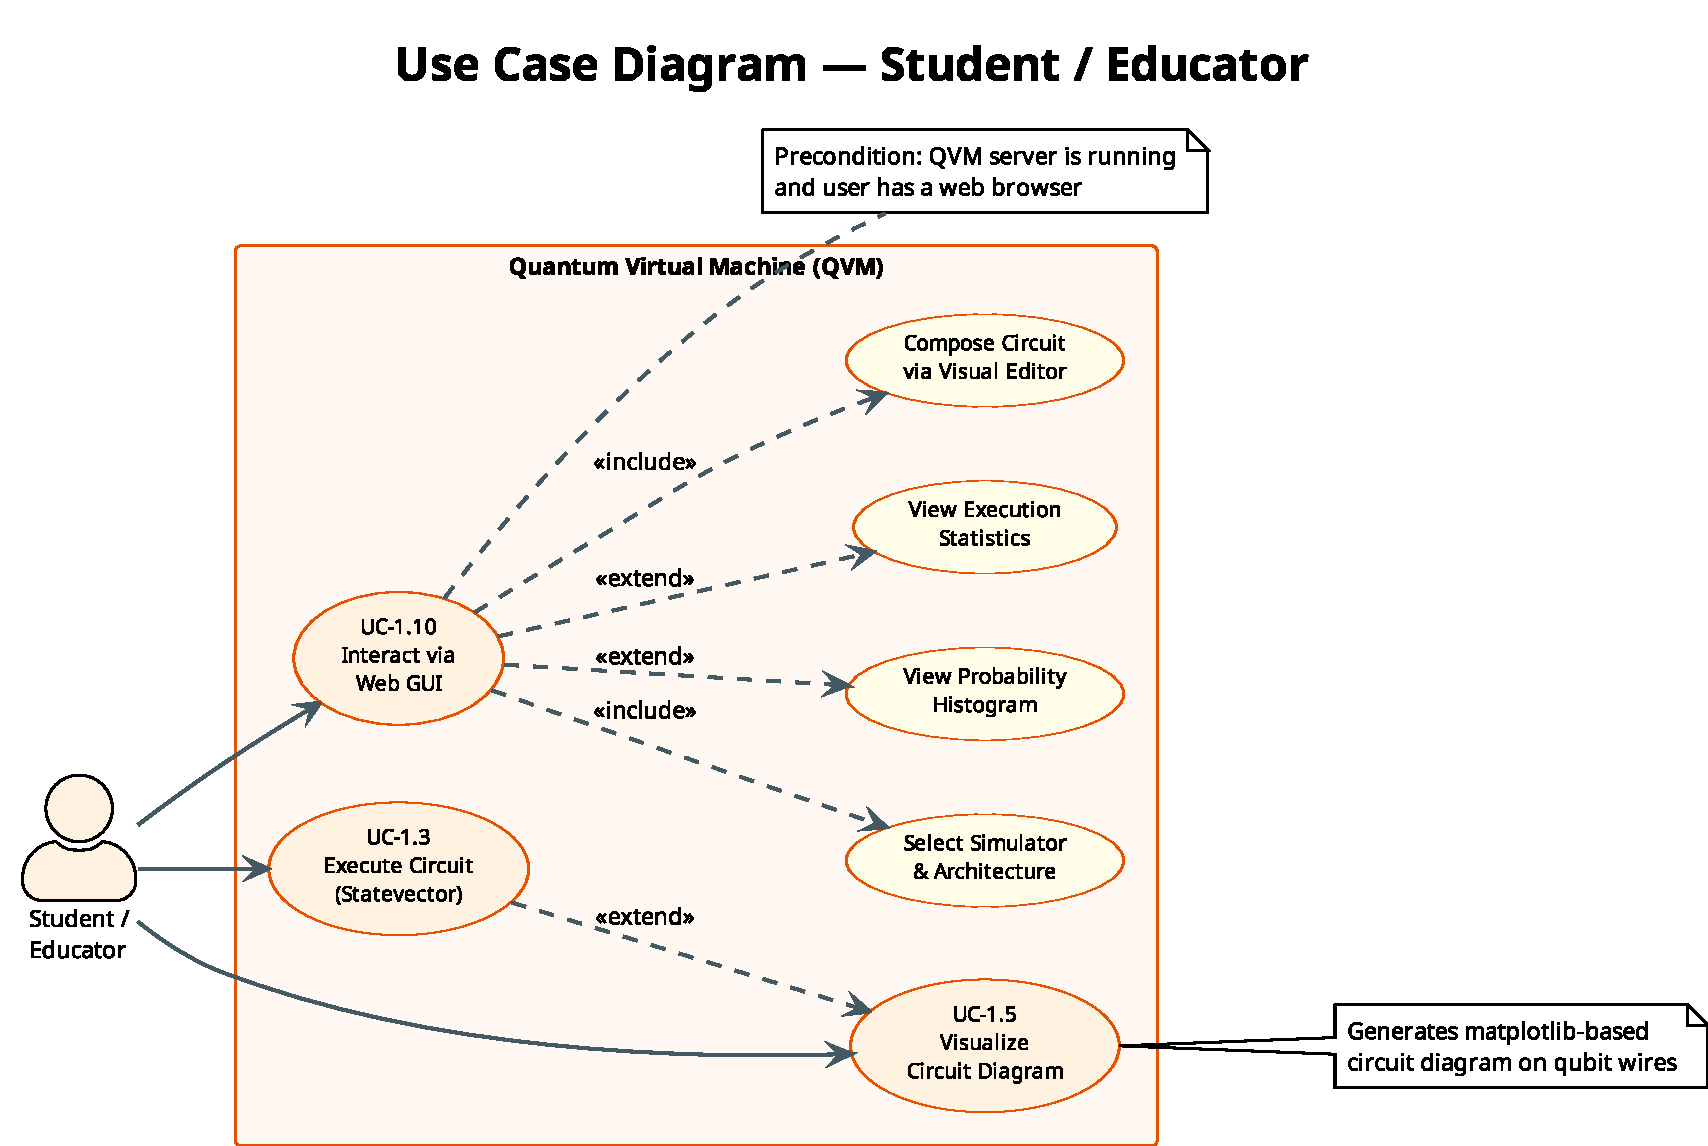
\includegraphics[width=0.9\textwidth,height=0.6\textheight,keepaspectratio]{../standalone_docs/figures/UC_Student.pdf}
\caption{Use Case Diagram --- Student / Educator}
\label{fig:uc_student}
\end{figure}

\subsubsection{Researcher}
Figure \ref{fig:uc_researcher} presents the use cases for the Researcher actor. This user class requires advanced simulation capabilities, including the MPS simulator and detailed transpilation benchmarking.

\begin{figure}[H]
\centering
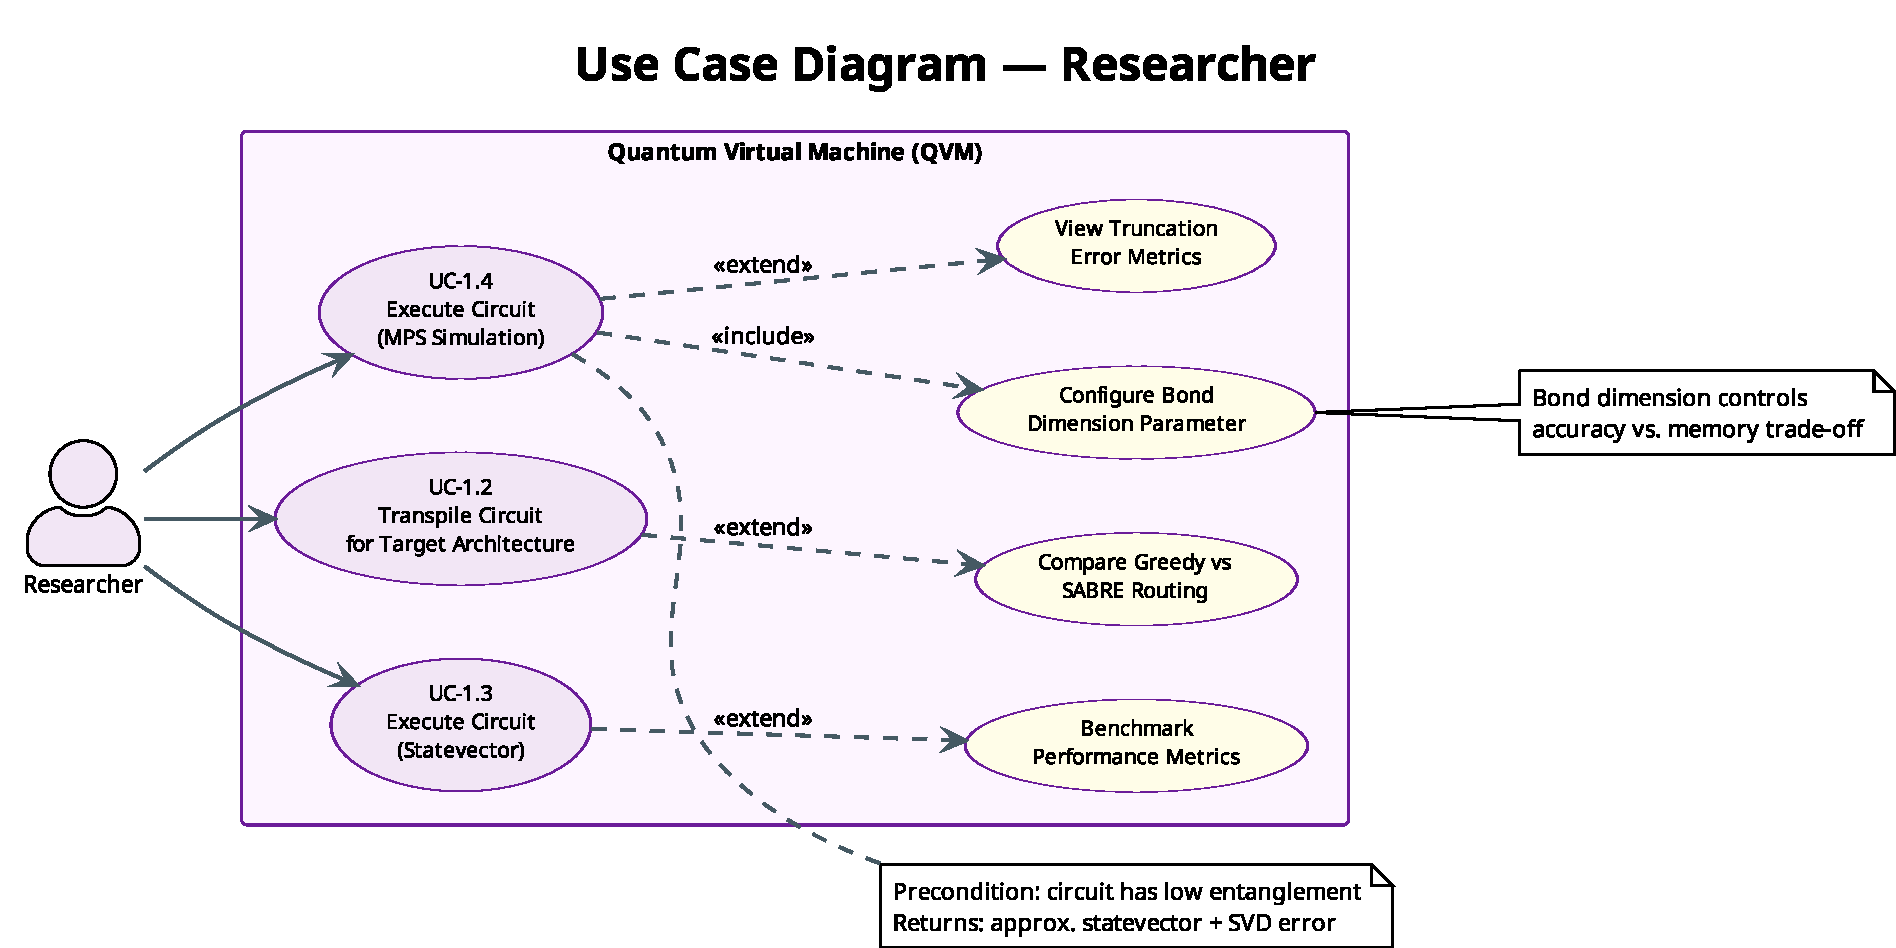
\includegraphics[width=0.9\textwidth,height=0.5\textheight,keepaspectratio]{../standalone_docs/figures/UC_Researcher.pdf}
\caption{Use Case Diagram --- Researcher}
\label{fig:uc_researcher}
\end{figure}

\subsubsection{System Integrator}
Figure \ref{fig:uc_integrator} depicts the use cases for the System Integrator actor. This actor accesses the QVM programmatically via the REST API or exports circuits in OpenQASM format for use with external quantum platforms.

\begin{figure}[H]
\centering
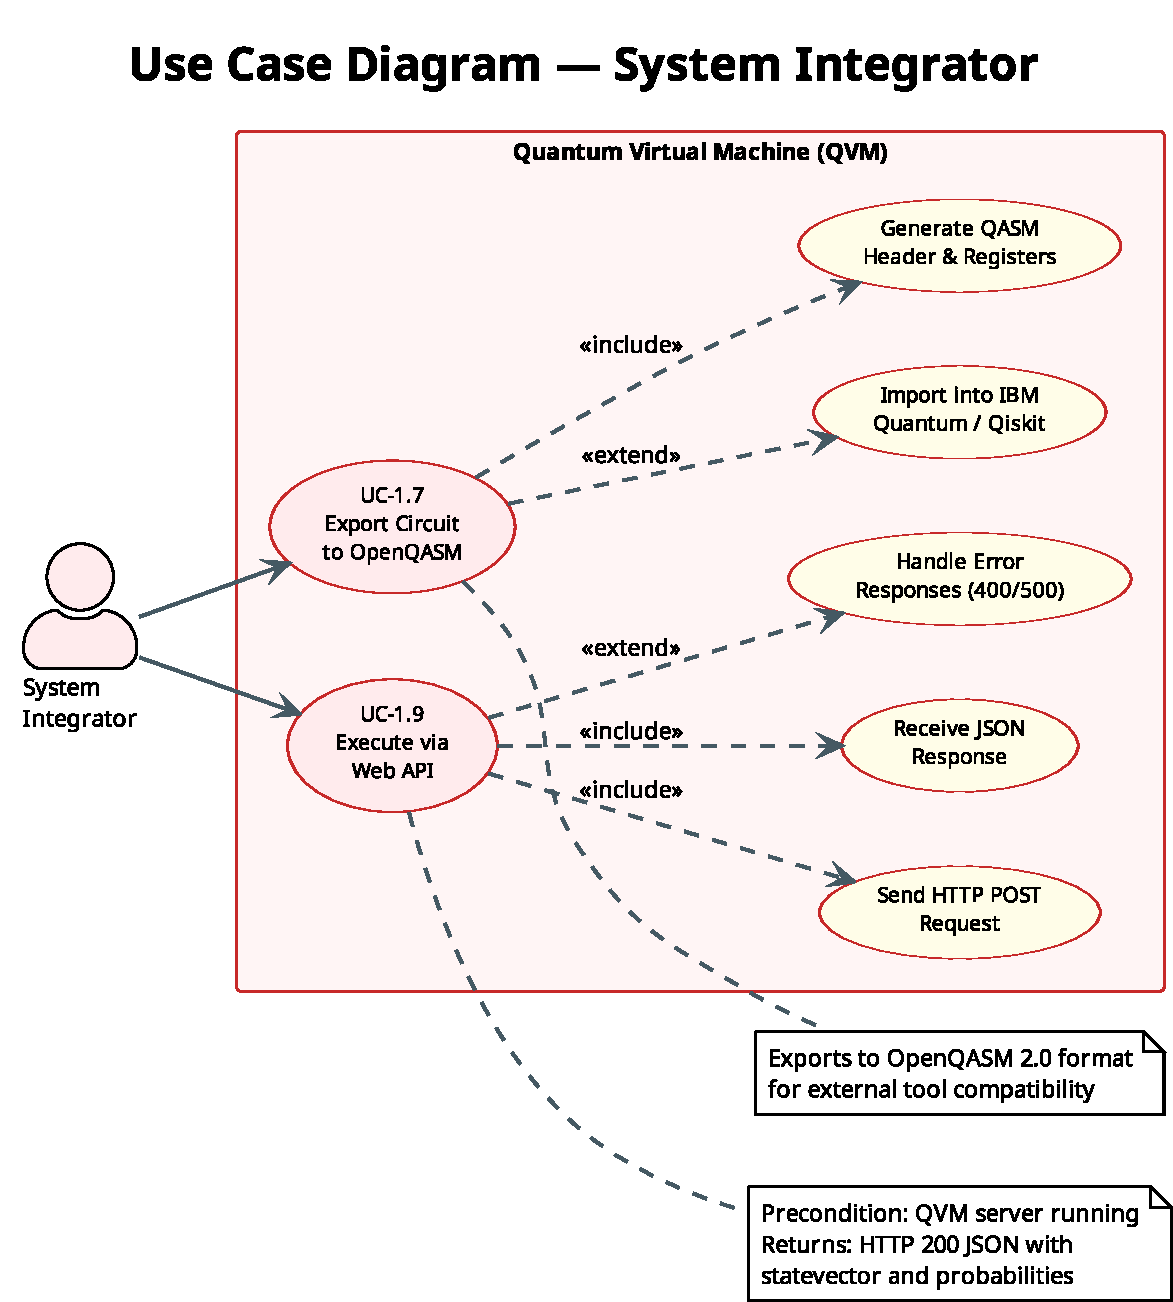
\includegraphics[width=0.9\textwidth,height=0.65\textheight,keepaspectratio]{../standalone_docs/figures/UC_Integrator.pdf}
\caption{Use Case Diagram --- System Integrator}
\label{fig:uc_integrator}
\end{figure}

\subsection{Use Case Descriptions}
The following descriptions provide detailed step-by-step flows for each use case identified in the diagram, including preconditions, main flows, and alternative paths.

\textbf{UC-1.1: Parse Quantum Circuit}
\begin{itemize}
\item \textbf{Actor:} Quantum Algorithm Developer
\item \textbf{Description:} User provides a quantum circuit in OpenQASM or JSON format, and the system parses it into an internal intermediate representation.
\item \textbf{Preconditions:} Valid circuit file exists
\item \textbf{Postconditions:} QuantumCircuit IR object is created
\item \textbf{Main Flow:}
\begin{enumerate}
\item User provides circuit file path
\item System detects file format (QASM 2.0, QASM 3.0, or JSON)
\item System invokes appropriate parser
\item Parser validates syntax and semantics
\item System creates QuantumCircuit IR object
\item System returns success confirmation
\end{enumerate}
\item \textbf{Alternative Flows:}
\begin{itemize}
\item 4a. Syntax error detected: System reports error with line number and description
\item 4b. Semantic error detected: System reports invalid gate or qubit reference
\end{itemize}
\end{itemize}

\textbf{UC-1.2: Transpile Circuit for Target Architecture}
\begin{itemize}
\item \textbf{Actor:} Quantum Algorithm Developer
\item \textbf{Description:} User requests transpilation of a logical circuit to match a specific hardware topology (e.g., linear chain, grid).
\item \textbf{Preconditions:} Valid QuantumCircuit IR exists; target architecture is defined
\item \textbf{Postconditions:} Physical circuit with SWAP gates inserted is generated
\item \textbf{Main Flow:}
\begin{enumerate}
\item User specifies target architecture and routing strategy
\item System analyzes circuit connectivity requirements
\item System applies routing algorithm (Greedy or SABRE)
\item System inserts SWAP gates to satisfy topology constraints
\item System optionally restores logical-to-physical mapping
\item System returns transpiled circuit
\end{enumerate}
\item \textbf{Alternative Flows:}
\begin{itemize}
\item 2a. Circuit requires more qubits than architecture provides: System reports error
\item 3a. No valid routing path exists: System reports disconnected topology error
\end{itemize}
\end{itemize}

\textbf{UC-1.3: Execute Circuit with Statevector Simulation}
\begin{itemize}
\item \textbf{Actor:} Quantum Algorithm Developer
\item \textbf{Description:} User executes a quantum circuit using exact statevector simulation.
\item \textbf{Preconditions:} Valid QuantumCircuit exists; circuit has $\leq 12$ qubits
\item \textbf{Postconditions:} Final statevector and measurement results are returned
\item \textbf{Main Flow:}
\begin{enumerate}
\item User initiates simulation
\item System initializes statevector to $|0\rangle^{\otimes n}$
\item System iterates through circuit operations
\item For each gate, system applies corresponding unitary matrix
\item For measurements, system performs probabilistic collapse
\item System returns final statevector and classical memory
\end{enumerate}
\item \textbf{Alternative Flows:}
\begin{itemize}
\item 1a. Circuit exceeds 12 qubits: System suggests MPS simulator
\item 3a. Infinite loop detected: System terminates after max operations limit
\end{itemize}
\end{itemize}

\textbf{UC-1.4: Execute Circuit with MPS Simulation}
\begin{itemize}
\item \textbf{Actor:} Researcher
\item \textbf{Description:} User executes a low-entanglement circuit using Matrix Product State simulation for efficiency.
\item \textbf{Preconditions:} Valid QuantumCircuit exists; circuit has low entanglement
\item \textbf{Postconditions:} Approximate statevector and measurement results are returned
\item \textbf{Main Flow:}
\begin{enumerate}
\item User initiates MPS simulation with bond dimension parameter
\item System initializes MPS representation
\item System applies gates using tensor contractions
\item System performs SVD truncation to maintain bond dimension
\item System returns final state and truncation error metrics
\end{enumerate}
\end{itemize}

\textbf{UC-1.5: Visualize Circuit}
\begin{itemize}
\item \textbf{Actor:} Student
\item \textbf{Description:} User requests a visual representation of the quantum circuit.
\item \textbf{Preconditions:} Valid QuantumCircuit exists
\item \textbf{Postconditions:} Circuit diagram is displayed or saved
\item \textbf{Main Flow:}
\begin{enumerate}
\item User requests visualization
\item System generates matplotlib-based circuit diagram
\item System displays gates on qubit wires with proper spacing
\item System shows measurement operations and classical bits
\item System renders diagram to screen or file
\end{enumerate}
\end{itemize}

\textbf{UC-1.6: Visualize Measurement Results}
\begin{itemize}
\item \textbf{Actor:} Quantum Algorithm Developer
\item \textbf{Description:} User requests a histogram of measurement outcome probabilities.
\item \textbf{Preconditions:} Circuit has been executed; statevector is available
\item \textbf{Postconditions:} Probability histogram is displayed
\item \textbf{Main Flow:}
\begin{enumerate}
\item User requests probability visualization
\item System computes $|\psi_i|^2$ for all basis states
\item System creates bar chart with basis states on x-axis
\item System displays probabilities on y-axis
\item System renders histogram to screen or file
\end{enumerate}
\end{itemize}

\textbf{UC-1.7: Export Circuit to OpenQASM}
\begin{itemize}
\item \textbf{Actor:} System Integrator
\item \textbf{Description:} User exports the internal circuit representation to OpenQASM 2.0 format for use with external tools.
\item \textbf{Preconditions:} Valid QuantumCircuit exists
\item \textbf{Postconditions:} OpenQASM string is generated
\item \textbf{Main Flow:}
\begin{enumerate}
\item User requests OpenQASM export
\item System generates QASM header with version and includes
\item System declares qubits and classical registers
\item System converts each operation to QASM syntax
\item System returns QASM string
\end{enumerate}
\end{itemize}

\textbf{UC-1.8: Execute via Command Line Interface}
\begin{itemize}
\item \textbf{Actor:} Quantum Algorithm Developer
\item \textbf{Description:} User runs a quantum circuit from the command line with various options.
\item \textbf{Preconditions:} QVM is installed; circuit file exists
\item \textbf{Postconditions:} Circuit is executed and results are displayed
\item \textbf{Main Flow:}
\begin{enumerate}
\item User invokes CLI with circuit file and options
\item System parses command-line arguments
\item System loads and parses circuit file
\item System applies optional transpilation
\item System executes circuit with specified simulator
\item System displays results and optional visualizations
\end{enumerate}
\end{itemize}

\textbf{UC-1.9: Execute via Web API}
\begin{itemize}
\item \textbf{Actor:} System Integrator
\item \textbf{Description:} User submits a circuit via HTTP POST request and receives JSON results.
\item \textbf{Preconditions:} QVM server is running
\item \textbf{Postconditions:} JSON response with results is returned
\item \textbf{Main Flow:}
\begin{enumerate}
\item User sends POST request with circuit JSON
\item Server validates request format
\item Server parses circuit
\item Server executes circuit
\item Server formats results as JSON
\item Server returns HTTP 200 with results
\end{enumerate}
\item \textbf{Alternative Flows:}
\begin{itemize}
\item 2a. Invalid JSON: Server returns HTTP 400 with error message
\item 4a. Execution error: Server returns HTTP 500 with error details
\end{itemize}
\end{itemize}

\textbf{UC-1.10: Interact via Web GUI}
\begin{itemize}
\item \textbf{Actor:} Student
\item \textbf{Description:} User composes and executes circuits through an interactive web dashboard.
\item \textbf{Preconditions:} QVM server is running; user has web browser
\item \textbf{Postconditions:} Circuit is executed and results are displayed in browser
\item \textbf{Main Flow:}
\begin{enumerate}
\item User accesses web interface
\item User composes circuit using visual editor or text input
\item User selects execution options (simulator, architecture)
\item User clicks execute button
\item System displays circuit diagram
\item System displays measurement results histogram
\item System shows execution statistics
\end{enumerate}
\end{itemize}

\section{Functional Requirements}

The functional requirements define the specific behaviors and capabilities that the QVM system must provide. These requirements are organized by the six major modules of the system architecture: Parsing and Input Processing, Intermediate Representation, Transpilation and Optimization, Simulation Engines, Visualization and Output, and User Interfaces. Each module's requirements specify the operations, validations, and transformations that the system must support to achieve its goal of hardware-agnostic quantum circuit execution.

\subsection{Module 1: Parsing and Input Processing}

The Parsing Module is responsible for converting quantum circuit descriptions from various input formats (OpenQASM 2.0, OpenQASM 3.0, JSON) into the system's internal intermediate representation. This module validates syntax, checks semantic correctness, and ensures that all gate operations and qubit references are well-formed before execution.

\begin{table}[H]
\centering
\caption{Functional Requirements - Parsing Module}
\begin{tabular}{|p{2cm}|p{11cm}|}
\hline
\textbf{Req. ID} & \textbf{Description} \\
\hline
FR-1.1 & The system shall parse OpenQASM 2.0 files with support for standard gates (h, x, y, z, cx, measure) \\
\hline
FR-1.2 & The system shall parse OpenQASM 3.0 files with support for control flow (if, for, while) and classical operations \\
\hline
FR-1.3 & The system shall parse JSON-formatted gate lists with gate names, qubits, and parameters \\
\hline
FR-1.4 & The system shall validate qubit indices to ensure they are within declared range \\
\hline
FR-1.5 & The system shall validate gate parameters (e.g., rotation angles) for correct data types \\
\hline
FR-1.6 & The system shall report syntax errors with line numbers and descriptive messages \\
\hline
FR-1.7 & The system shall support classical register declarations (bit, bit[n]) \\
\hline
FR-1.8 & The system shall support qubit register declarations (qubit, qubit[n]) \\
\hline
\end{tabular}
\end{table}

\subsection{Module 2: Intermediate Representation}

The Intermediate Representation (IR) Module provides a unified data structure for representing quantum circuits internally. This module supports quantum operations, classical registers, conditional execution, control flow primitives (labels and jumps), and classical bit operations, enabling the system to handle both pure quantum algorithms and hybrid quantum-classical programs.

\begin{table}[H]
\centering
\caption{Functional Requirements - IR Module}
\begin{tabular}{|p{2cm}|p{11cm}|}
\hline
\textbf{Req. ID} & \textbf{Description} \\
\hline
FR-2.1 & The system shall represent quantum circuits as a QuantumCircuit object with num\_qubits and operations list \\
\hline
FR-2.2 & The system shall store operations as dictionaries containing gate name, qubits, parameters, and conditions \\
\hline
FR-2.3 & The system shall support conditional operations with register, index, and value specifications \\
\hline
FR-2.4 & The system shall support measurement operations with target classical bit specification \\
\hline
FR-2.5 & The system shall support label and jump operations for control flow \\
\hline
FR-2.6 & The system shall support classical operations (assignment, AND, OR, XOR, NOT) \\
\hline
FR-2.7 & The system shall support delay operations with duration specifications \\
\hline
FR-2.8 & The system shall provide string representation of circuits for debugging \\
\hline
\end{tabular}
\end{table}

\subsection{Module 3: Transpilation and Optimization}

The Transpilation Module performs hardware-aware circuit compilation, mapping logical quantum circuits to physical hardware topologies with connectivity constraints. This module implements routing algorithms (Greedy BFS and SABRE) that insert SWAP gates to satisfy topology requirements while minimizing circuit depth and maintaining logical equivalence.

\begin{table}[H]
\centering
\caption{Functional Requirements - Transpiler Module}
\begin{tabular}{|p{2cm}|p{11cm}|}
\hline
\textbf{Req. ID} & \textbf{Description} \\
\hline
FR-3.1 & The system shall support Greedy BFS routing strategy for qubit mapping \\
\hline
FR-3.2 & The system shall support SABRE routing strategy with lookahead heuristics \\
\hline
FR-3.3 & The system shall insert SWAP gates to satisfy topology connectivity constraints \\
\hline
FR-3.4 & The system shall support linear chain topology (qubits connected in a line) \\
\hline
FR-3.5 & The system shall support grid topology (qubits connected in 2D lattice) \\
\hline
FR-3.6 & The system shall optionally restore logical-to-physical qubit mapping after transpilation \\
\hline
FR-3.7 & The system shall validate that logical circuit fits within target architecture qubit count \\
\hline
FR-3.8 & The system shall cache distance calculations for performance optimization \\
\hline
FR-3.9 & The system shall decompose complex gates (Toffoli) into native gate sets \\
\hline
FR-3.10 & The system shall preserve single-qubit gates without modification during transpilation \\
\hline
\end{tabular}
\end{table}

\subsection{Module 4: Simulation Engines}

The Simulation Module executes quantum circuits using statevector evolution or tensor network methods. This module supports exact simulation for circuits up to 12 qubits using full statevector representation, and approximate simulation for larger low-entanglement circuits using Matrix Product State (MPS) decomposition with configurable bond dimensions.

\begin{table}[H]
\centering
\caption{Functional Requirements - Simulator Module}
\begin{tabular}{|p{2cm}|p{11cm}|}
\hline
\textbf{Req. ID} & \textbf{Description} \\
\hline
FR-4.1 & The system shall simulate circuits using exact statevector evolution for up to 12 qubits \\
\hline
FR-4.2 & The system shall support single-qubit gates (H, X, Y, Z, Rx, Ry, Rz, S, T, SX) \\
\hline
FR-4.3 & The system shall support two-qubit gates (CX, SWAP) \\
\hline
FR-4.4 & The system shall support three-qubit gates (CCX/Toffoli) \\
\hline
FR-4.5 & The system shall perform measurements with probabilistic state collapse \\
\hline
FR-4.6 & The system shall maintain classical memory registers synchronized with quantum state \\
\hline
FR-4.7 & The system shall support conditional gate execution based on classical bit values \\
\hline
FR-4.8 & The system shall support control flow (labels, jumps, loops) with infinite loop detection \\
\hline
FR-4.9 & The system shall support MPS simulation for low-entanglement circuits with configurable bond dimension \\
\hline
FR-4.10 & The system shall report truncation error for MPS simulations \\
\hline
FR-4.11 & The system shall use NumPy vectorization for efficient matrix operations \\
\hline
FR-4.12 & The system shall support seeded random number generation for reproducible measurements \\
\hline
\end{tabular}
\end{table}

\subsection{Module 5: Visualization and Output}

The Visualization Module generates graphical representations of quantum circuits and measurement results. This module creates circuit diagrams showing gate operations on qubit wires, probability histograms for measurement outcomes, and exports circuits to OpenQASM 2.0 format for interoperability with external quantum computing platforms.

\begin{table}[H]
\centering
\caption{Functional Requirements - Visualization Module}
\begin{tabular}{|p{2cm}|p{11cm}|}
\hline
\textbf{Req. ID} & \textbf{Description} \\
\hline
FR-5.1 & The system shall generate circuit diagrams using matplotlib with gates on qubit wires \\
\hline
FR-5.2 & The system shall display measurement operations with classical bit targets \\
\hline
FR-5.3 & The system shall generate probability histograms for measurement outcomes \\
\hline
FR-5.4 & The system shall export circuits to OpenQASM 2.0 format \\
\hline
FR-5.5 & The system shall save visualizations to PNG files \\
\hline
FR-5.6 & The system shall display execution statistics (circuit depth, gate count) \\
\hline
\end{tabular}
\end{table}

\subsection{Module 6: User Interfaces}

The User Interface Module provides three access methods for interacting with the QVM system: a command-line interface for scripting and automation, a RESTful web API for programmatic access, and a browser-based graphical interface for interactive circuit composition and execution. These interfaces accommodate different user workflows from batch processing to educational exploration.

\begin{table}[H]
\centering
\caption{Functional Requirements - Interface Module}
\begin{tabular}{|p{2cm}|p{11cm}|}
\hline
\textbf{Req. ID} & \textbf{Description} \\
\hline
FR-6.1 & The system shall provide a command-line interface accepting file paths and options \\
\hline
FR-6.2 & The system shall support CLI flags for transpilation (--transpile, --routing, --architecture) \\
\hline
FR-6.3 & The system shall support CLI flags for simulation (--simulator, --shots, --seed) \\
\hline
FR-6.4 & The system shall provide a REST API with POST /execute endpoint \\
\hline
FR-6.5 & The system shall accept JSON circuit definitions via API \\
\hline
FR-6.6 & The system shall return JSON responses with statevector, probabilities, and metadata \\
\hline
FR-6.7 & The system shall provide a web GUI with circuit editor \\
\hline
FR-6.8 & The system shall display real-time execution results in web GUI \\
\hline
FR-6.9 & The system shall provide example circuits in web GUI \\
\hline
\end{tabular}
\end{table}

\section{Non-Functional Requirements}

Non-functional requirements define the quality attributes and constraints that the QVM system must satisfy. These requirements ensure that the system not only provides the correct functionality but also meets standards for performance, reliability, usability, portability, maintainability, and security. The following subsections detail the specific non-functional requirements across these six quality dimensions.

\subsection{Performance Requirements}

Performance requirements specify the execution speed and resource efficiency that the system must achieve. These requirements ensure that the QVM can simulate quantum circuits within acceptable time bounds on standard computing hardware, making it practical for educational use and algorithm development.

\begin{table}[H]
\centering
\caption{Non-Functional Requirements - Performance}
\begin{tabular}{|p{2cm}|p{11cm}|}
\hline
\textbf{Req. ID} & \textbf{Description} \\
\hline
NFR-1.1 & The system shall simulate 10-qubit circuits in under 5 seconds on standard hardware \\
\hline
NFR-1.2 & The system shall parse OpenQASM 3.0 files in under 1 second for circuits with up to 1000 operations \\
\hline
NFR-1.3 & The system shall transpile circuits with under 100 gates in under 2 seconds using SABRE routing \\
\hline
NFR-1.4 & The system shall support MPS simulation of 20-qubit low-entanglement circuits \\
\hline
NFR-1.5 & The system shall cache distance calculations to avoid redundant BFS searches \\
\hline
\end{tabular}
\end{table}

\subsection{Reliability Requirements}

Reliability requirements define the system's ability to handle errors gracefully and maintain correct operation under various conditions. These requirements ensure that the QVM validates inputs, detects potential issues like infinite loops, and provides clear diagnostic information when problems occur.

\begin{table}[H]
\centering
\caption{Non-Functional Requirements - Reliability}
\begin{tabular}{|p{2cm}|p{11cm}|}
\hline
\textbf{Req. ID} & \textbf{Description} \\
\hline
NFR-2.1 & The system shall detect and prevent infinite loops in control flow with configurable operation limits \\
\hline
NFR-2.2 & The system shall validate all input circuits before execution \\
\hline
NFR-2.3 & The system shall provide descriptive error messages for all failure modes \\
\hline
NFR-2.4 & The system shall maintain numerical stability for statevector normalization \\
\hline
NFR-2.5 & The system shall achieve 95\% test coverage with automated unit tests \\
\hline
\end{tabular}
\end{table}

\subsection{Usability Requirements}

Usability requirements specify the ease of use and learnability of the system for different user classes. These requirements ensure that the QVM provides clear documentation, intuitive interfaces, and helpful examples that enable users to quickly understand and effectively use the system for quantum algorithm development and education.

\begin{table}[H]
\centering
\caption{Non-Functional Requirements - Usability}
\begin{tabular}{|p{2cm}|p{11cm}|}
\hline
\textbf{Req. ID} & \textbf{Description} \\
\hline
NFR-3.1 & The system shall provide comprehensive documentation with usage examples \\
\hline
NFR-3.2 & The system shall provide clear CLI help messages with --help flag \\
\hline
NFR-3.3 & The system shall provide example circuits for common algorithms (Bell, GHZ, Grover) \\
\hline
NFR-3.4 & The system shall use intuitive gate naming conventions consistent with Qiskit \\
\hline
NFR-3.5 & The web GUI shall be accessible without installation via web browser \\
\hline
\end{tabular}
\end{table}

\subsection{Portability Requirements}

Portability requirements define the system's ability to run on different operating systems and integrate with external quantum computing platforms. These requirements ensure that the QVM can be deployed across Windows, Linux, and macOS environments, and can exchange circuit definitions with industry-standard tools through OpenQASM format support.

\begin{table}[H]
\centering
\caption{Non-Functional Requirements - Portability}
\begin{tabular}{|p{2cm}|p{11cm}|}
\hline
\textbf{Req. ID} & \textbf{Description} \\
\hline
NFR-4.1 & The system shall run on Windows, Linux, and macOS operating systems \\
\hline
NFR-4.2 & The system shall require only Python 3.10+ and standard scientific libraries \\
\hline
NFR-4.3 & The system shall export circuits to OpenQASM 2.0 for compatibility with IBM Quantum \\
\hline
NFR-4.4 & The system shall support multiple input formats (QASM 2.0, QASM 3.0, JSON) \\
\hline
\end{tabular}
\end{table}

\subsection{Maintainability Requirements}

Maintainability requirements specify the code quality standards and development practices that facilitate future modifications and extensions. These requirements ensure that the QVM codebase is well-documented, follows consistent coding conventions, and uses modular design principles that enable developers to understand, modify, and extend the system efficiently.

\begin{table}[H]
\centering
\caption{Non-Functional Requirements - Maintainability}
\begin{tabular}{|p{2cm}|p{11cm}|}
\hline
\textbf{Req. ID} & \textbf{Description} \\
\hline
NFR-5.1 & The system shall follow modular architecture with clear separation of concerns \\
\hline
NFR-5.2 & The system shall include docstrings for all public functions and classes \\
\hline
NFR-5.3 & The system shall use type hints for function signatures \\
\hline
NFR-5.4 & The system shall maintain version control with Git \\
\hline
NFR-5.5 & The system shall follow PEP 8 Python style guidelines \\
\hline
\end{tabular}
\end{table}

\subsection{Security Requirements}

Security requirements define the system's protection mechanisms against malicious inputs and resource exhaustion attacks. These requirements ensure that the QVM validates all user inputs, prevents directory traversal vulnerabilities, and implements resource limits to protect against denial-of-service attempts while maintaining usability for legitimate users.

\begin{table}[H]
\centering
\caption{Non-Functional Requirements - Security}
\begin{tabular}{|p{2cm}|p{11cm}|}
\hline
\textbf{Req. ID} & \textbf{Description} \\
\hline
NFR-6.1 & The system shall validate all file paths to prevent directory traversal attacks \\
\hline
NFR-6.2 & The system shall sanitize user input in web API to prevent injection attacks \\
\hline
NFR-6.3 & The system shall limit maximum circuit size to prevent resource exhaustion \\
\hline
NFR-6.4 & The system shall implement operation count limits to prevent denial-of-service \\
\hline
\end{tabular}
\end{table}
\FloatBarrier

\section{External Interface Requirements}

External interface requirements specify how the QVM system interacts with users, hardware, software components, and external systems. These requirements define the boundaries of the system and the protocols for communication across those boundaries. The following subsections detail the user interfaces, hardware interfaces, software dependencies, and communication protocols that the system must support.

\subsection{User Interfaces}
The system provides three user interfaces:

\textbf{Command-Line Interface (CLI):} A terminal-based interface accepting file paths and command-line flags. Supports batch processing and scripting. Displays text-based output with optional visualization windows.

\textbf{Web API:} A RESTful HTTP API built with FastAPI. Accepts JSON POST requests at /execute endpoint. Returns JSON responses with statevector, probabilities, and execution metadata. Supports CORS for cross-origin requests.

\textbf{Web GUI:} A browser-based dashboard with circuit editor, execution controls, and result visualization. Built with HTML/CSS/JavaScript. Communicates with backend via REST API. Displays circuit diagrams and probability histograms inline.

\subsection{Hardware Interfaces}
The system runs on standard computing hardware with the following minimum specifications:
\begin{itemize}
\item CPU: Dual-core processor (2.0 GHz or higher)
\item RAM: 4 GB minimum (8 GB recommended for 12-qubit circuits)
\item Storage: 100 MB for installation
\item Display: 1024x768 resolution for GUI
\end{itemize}

\subsection{Software Interfaces}
The system interfaces with the following software components:

\textbf{Python Runtime:} Requires Python 3.10 or higher for execution.

\textbf{NumPy:} Used for linear algebra operations (matrix multiplication, tensor products). Version 1.21+ required.

\textbf{Matplotlib:} Used for visualization (circuit diagrams, histograms). Version 3.5+ required.

\textbf{Lark:} Used for OpenQASM 3.0 parsing with LALR parser. Version 1.1+ required.

\textbf{FastAPI:} Used for web API server. Version 0.95+ required.

\textbf{Uvicorn:} ASGI server for running FastAPI application.

\subsection{Communication Interfaces}
The system uses the following communication protocols:

\textbf{HTTP/HTTPS:} Web API communicates via HTTP POST requests with JSON payloads. Supports standard HTTP status codes (200, 400, 500).

\textbf{File I/O:} Reads circuit files from local filesystem. Supports .qasm, .json file extensions. Writes visualization outputs to .png files.

\textbf{Standard I/O:} CLI uses stdin for input and stdout/stderr for output. Supports piping and redirection.

\section{Requirement Traceability Matrix}

\begin{table}[H]
\centering
\caption{Requirement Traceability Matrix}
\begin{tabular}{|p{2.5cm}|p{4cm}|p{6cm}|}
\hline
\textbf{Business Objective} & \textbf{Functional Requirements} & \textbf{Use Cases} \\
\hline
BO-1: Hardware Agnosticism & FR-3.1, FR-3.2, FR-3.3, FR-3.4, FR-3.5 & UC-1.2 \\
\hline
BO-2: Educational Value & FR-5.1, FR-5.2, FR-5.3, FR-6.7, FR-6.9 & UC-1.5, UC-1.6, UC-1.10 \\
\hline
BO-3: Lightweight Runtime & FR-4.1, FR-4.11, NFR-1.1, NFR-4.2 & UC-1.3 \\
\hline
BO-4: Interoperability & FR-1.1, FR-1.2, FR-5.4, NFR-4.3 & UC-1.1, UC-1.7 \\
\hline
BO-5: Flexibility & FR-2.3, FR-2.5, FR-2.6, FR-4.7, FR-4.8 & UC-1.3, UC-1.4 \\
\hline
\end{tabular}
\end{table}
\FloatBarrier

\section{Summary}
This chapter has presented a comprehensive analysis of the Quantum Virtual Machine requirements, covering functional requirements across six major modules (Parsing, IR, Transpilation, Simulation, Visualization, Interfaces) and non-functional requirements across six quality attributes (Performance, Reliability, Usability, Portability, Maintainability, Security). The requirements were elicited through literature review, comparative analysis, and iterative prototyping. Ten detailed use cases were documented, covering the primary user interactions with the system, with individual use case diagrams provided for each of the four user classes: Quantum Algorithm Developer, Student/Educator, Researcher, and System Integrator. The requirement traceability matrix demonstrates clear alignment between business objectives and functional requirements. These requirements guided the system design and implementation, ensuring that the QVM achieves its goal of providing a hardware-agnostic, educational, and lightweight quantum execution runtime.


\end{document}
